\chapter{Augmented via Additive}\label{chap:3}

\begin{figure}[H]
    \centering
    
\includegraphics[width=1\linewidth]{figures/chapter 3/ch3_A.pdf}
    \caption[Augmented via Additive "A"]{\textbf{Augmented via Additive "A" } Visual representation of the "Augmented via Additive" strategy, highlighting the integration of additive manufacturing techniques (e.g., 3D printing) into scaffold fabrication workflows to enhance mechanical performance, structural precision, and design versatility in tissue engineering applications. }
    \label{fig:ch3_A}
\end{figure}

\section{``Augmented via Additive'': Leveraging 3D Printing for Enhanced Scaffold Development}

The ``augmented via additive'' approach reflects a dual strategy: first, the use of additive manufacturing to develop precision-engineered mechanical testing equipment that overcomes the limitations of traditional hydrogel characterization; and second, the reinforcement of hydrogels through additively manufactured PCL networks to enhance mechanical performance. 

Before advancing to scaffold reinforcement, it was essential to establish accurate baseline mechanical characterization of the hydrogel components. Conventional mechanical testing methods often fail to capture the complex poroviscoelastic behavior of hydrated, low-modulus biomaterials. Additive manufacturing provided a transformative solution, enabling rapid prototyping of a custom confined compression chamber with high precision, transparent materials for visual monitoring, and design features unattainable through traditional machining. This platform established a robust foundation for subsequent scaffold development and validation.

\section{Testing and Characterization Challenges}

Accurately characterizing the mechanical behavior of hydrated, low-modulus biomaterials like gelatin-based hydrogels presents significant challenges in meniscal tissue engineering. Traditional mechanical testing systems often fail to capture the complex poroviscoelastic behavior of these highly hydrated scaffolds \cite{chaudhuri2016hydrogelstunable, roberts2011comparativestudy, nichol2010cellviability, antoine2014review}. These challenges stem from both intrinsic material properties (high water content, low modulus) and limitations of conventional testing platforms.

Recent advances in mechanical testing methodologies have enabled more accurate assessment of soft biomaterials' poroviscoelastic properties and better correlation with in vivo performance~\cite{nelson2024methodstesting}. The development of depth-dependent reinforcement strategies has been particularly important for creating scaffolds with controlled mechanical properties~\cite{chendepthstraindependent}.

The distinction between confined and unconfined compression testing is critical for understanding hydrated biomaterial behavior~\cite{bursaconnedunconned}. Confined compression, which restricts radial displacement, better simulates the in vivo loading environment where anatomical constraints prevent lateral expansion. An in-depth understanding of testing approaches is essential for developing reliable characterization protocols~\cite{carterindepthguide}.

In our initial characterization using unconfined compression, we identified significant limitations. The hydrogels exhibited substantial lateral expansion during compression, leading to slippage at platen interfaces and unstable force readings. Moreover, the unconfined setup failed to accurately replicate the constrained mechanical environment of native meniscal tissue. These challenges motivated our transition toward confined compression testing to achieve more reliable and physiologically relevant measurements.

Confined compression setups, typically designed for bulk materials, present key obstacles: misalignment between platens and samples leads to edge effects and non-uniform loading; small chamber sizes (3--10 mm diameter) yield weak force signals and poor signal-to-noise ratios; and friction between samples and chamber walls distorts true material response. Additionally, lack of environmental controls often results in sample dehydration and compromised data integrity. Early tests using commercial and ad hoc systems yielded inconsistent results, underscoring the need for a purpose-built platform capable of precise alignment, rigid confinement, uniform drainage, and continuous hydration.

\begin{figure}[H]
    \centering
    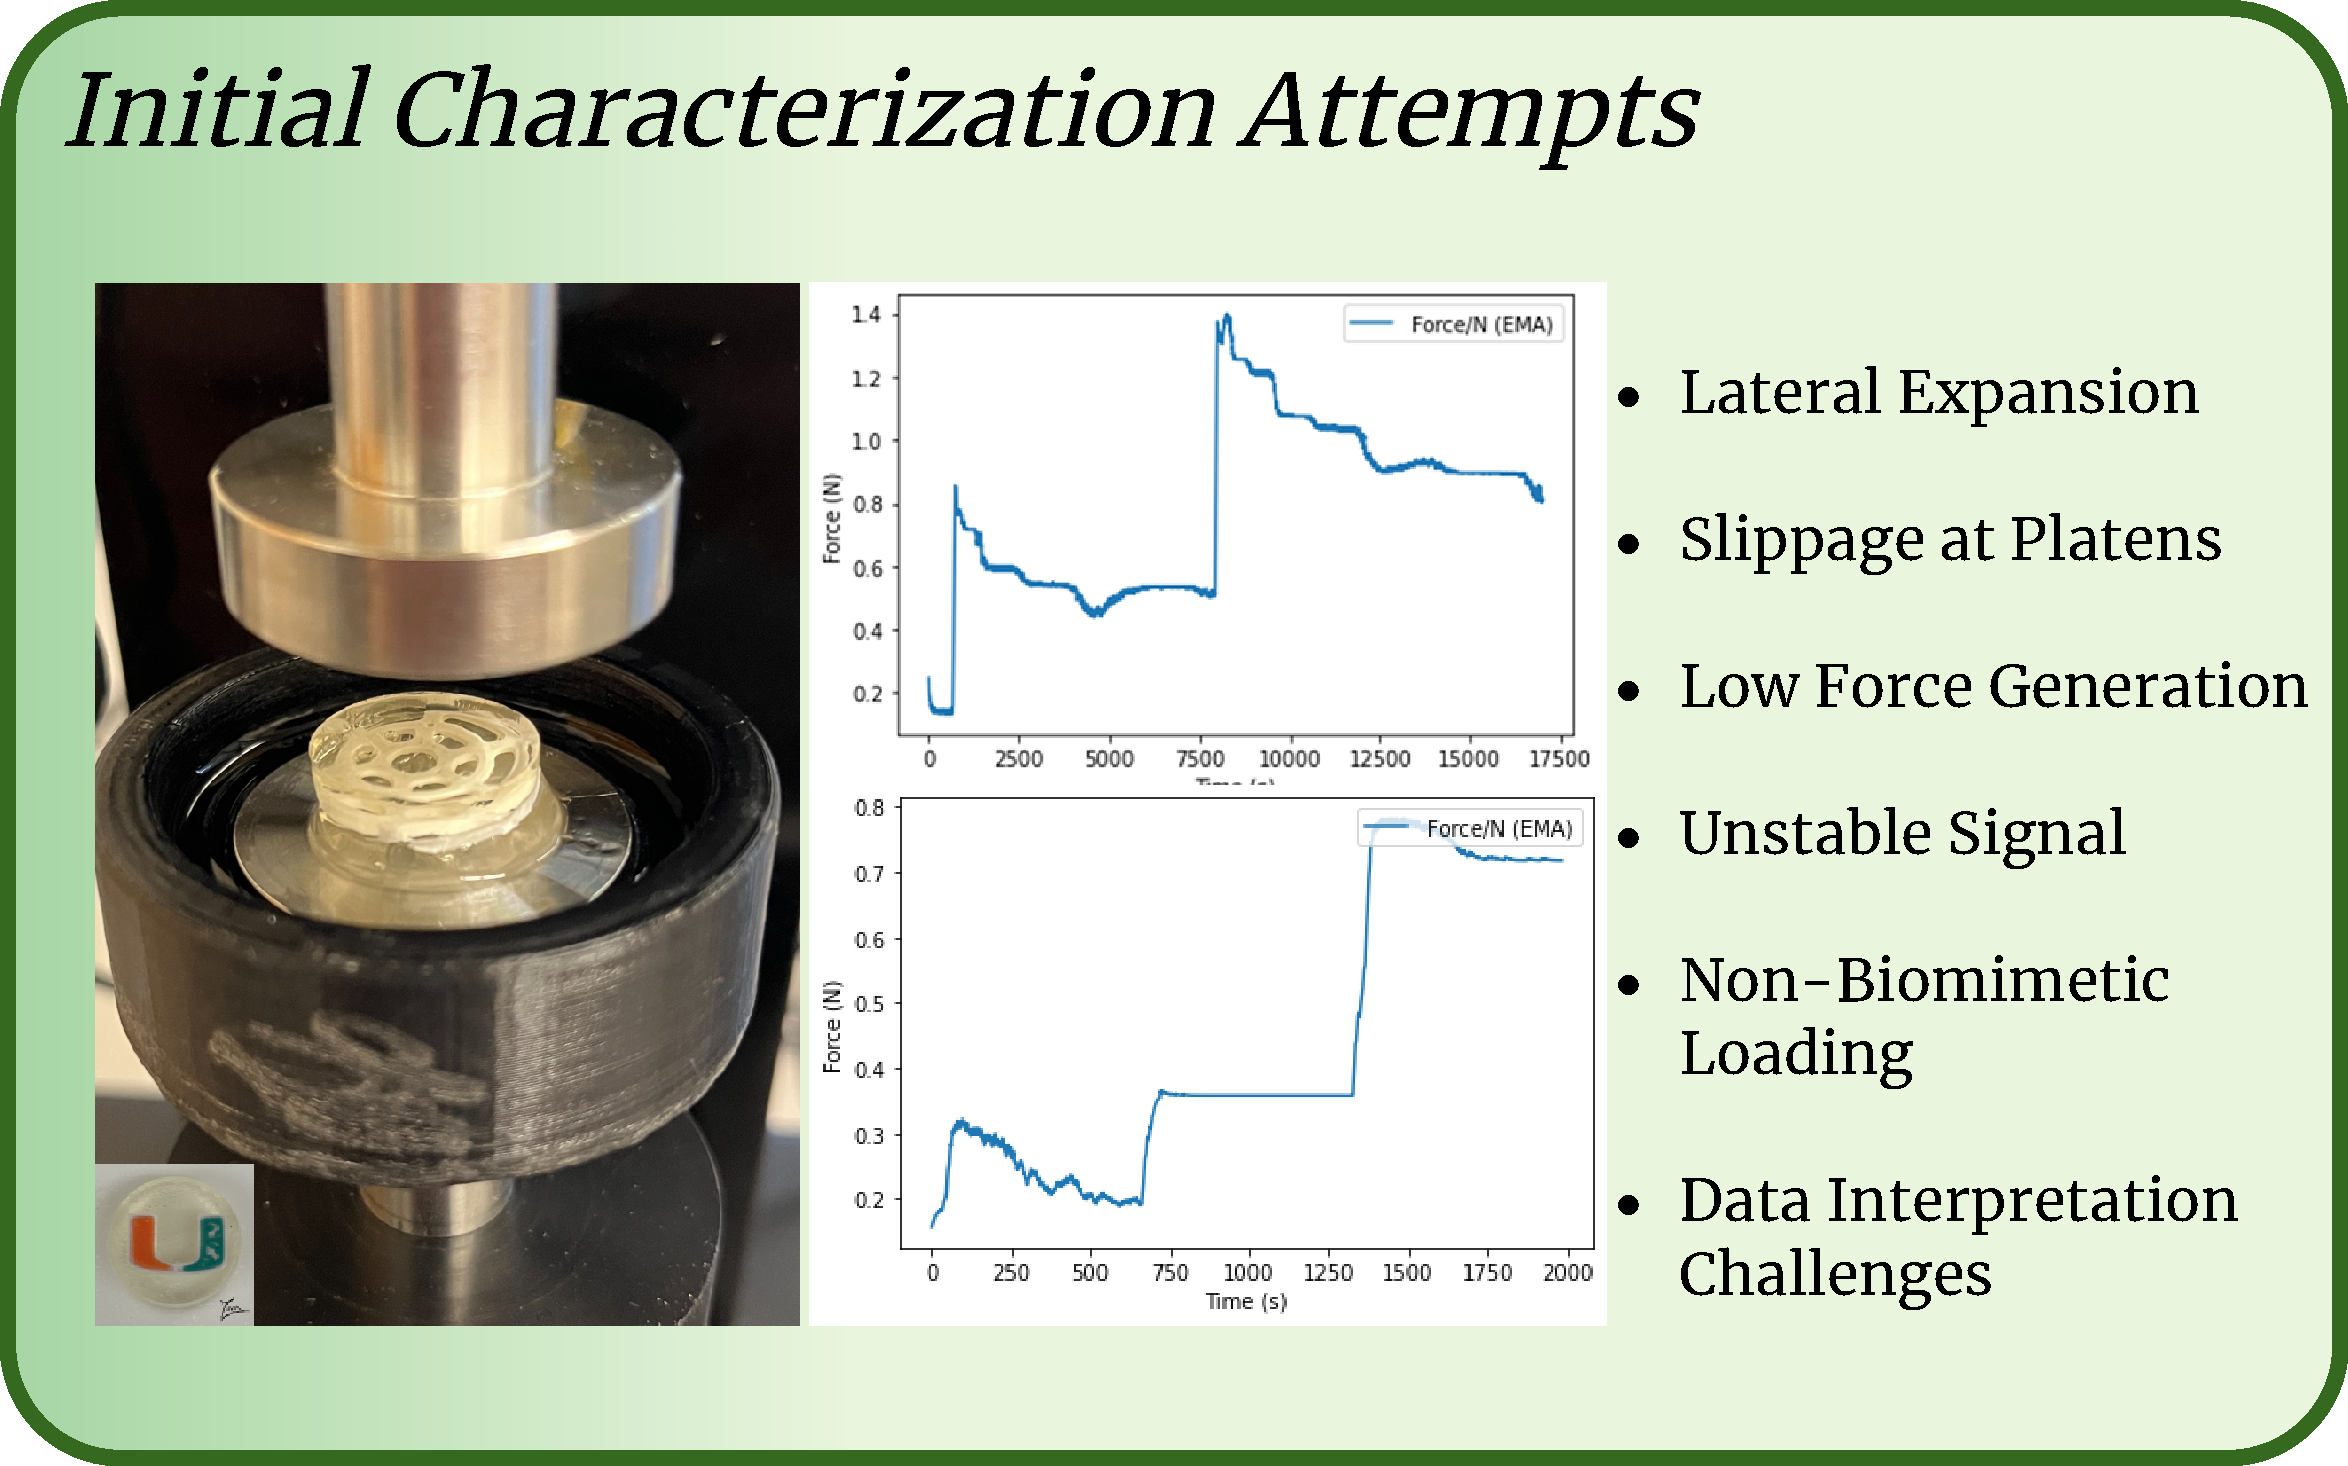
\includegraphics[width=1\linewidth]{figures/chapter 3/ch3_unconfinedEarly.pdf}
    \caption[Initial unconfined compression testing of hydrogel scaffolds]{\textbf{Initial unconfined compression testing of hydrogel scaffolds.} The setup (left) shows the hydrogel sample positioned between compression platens, while force–time plots (right) illustrate unstable and low-force responses characteristic of early testing attempts. Key challenges included lateral expansion, slippage at platen interfaces, and non-biomimetic loading, all of which hindered reliable mechanical characterization. }
    \label{fig:ch3_unconfined}
\end{figure}


To assess hydrogel mechanical performance under physiologically relevant conditions, stress-relaxation testing was employed, where samples are compressed to a fixed strain while stress decay over time reflects the scaffold's ability to dissipate mechanical energy \cite{watasestressrelaxation, makris2011kneemeniscus}. GelA--GTA hydrogels exhibit poroviscoelastic responses strongly influenced by crosslinking density and hydration state \cite{chaudhuri2016hydrogelstunable, morejon2020compressiveproperties}, necessitating precise and reproducible testing protocols as we examine the theoretical framework underpinning compression testing methods and their implications for accurate mechanical evaluation.

\clearpage
\subsection{Theoretical Framework: \protect\\ Unconfined vs. Confined Compression Testing}

Two primary modes characterize soft biomaterials: unconfined and confined compression, both derived from poroelastic theory where mechanical response results from fluid flow and solid matrix deformation.

\subsubsection{Unconfined Compression}

In unconfined compression, samples are compressed axially while allowed to expand radially, mimicking physiological deformation but introducing complexity through multi-directional fluid flow. Boundary conditions include radial displacement ($u_r \neq 0$) and pore pressure allowing fluid to exit both radially and axially. The characteristic relaxation time scales with sample radius squared ($\tau \sim a^2$), emphasizing how radial drainage determines time-dependent behavior.

\subsubsection{Confined Compression}

Confined compression restricts radial displacement ($u_r = 0$), forcing fluid to drain axially through porous platens. This simulates constrained environments like the meniscus under load, where rigid anatomical structures prevent lateral expansion. The theoretical framework relies on perfect confinement with no radial movement, uniform axial drainage with pore pressure $p = 0$ at platen interfaces, and smooth, rigid chamber walls to prevent wall deformation or frictional effects. Under these conditions, the characteristic relaxation time scales with sample thickness squared ($\tau \sim h^2$), indicating that stress relaxation rate is determined by fluid travel distance rather than lateral dimensions.

\subsection{Stress Relaxation Testing}

\begin{figure}[H]
    \centering
    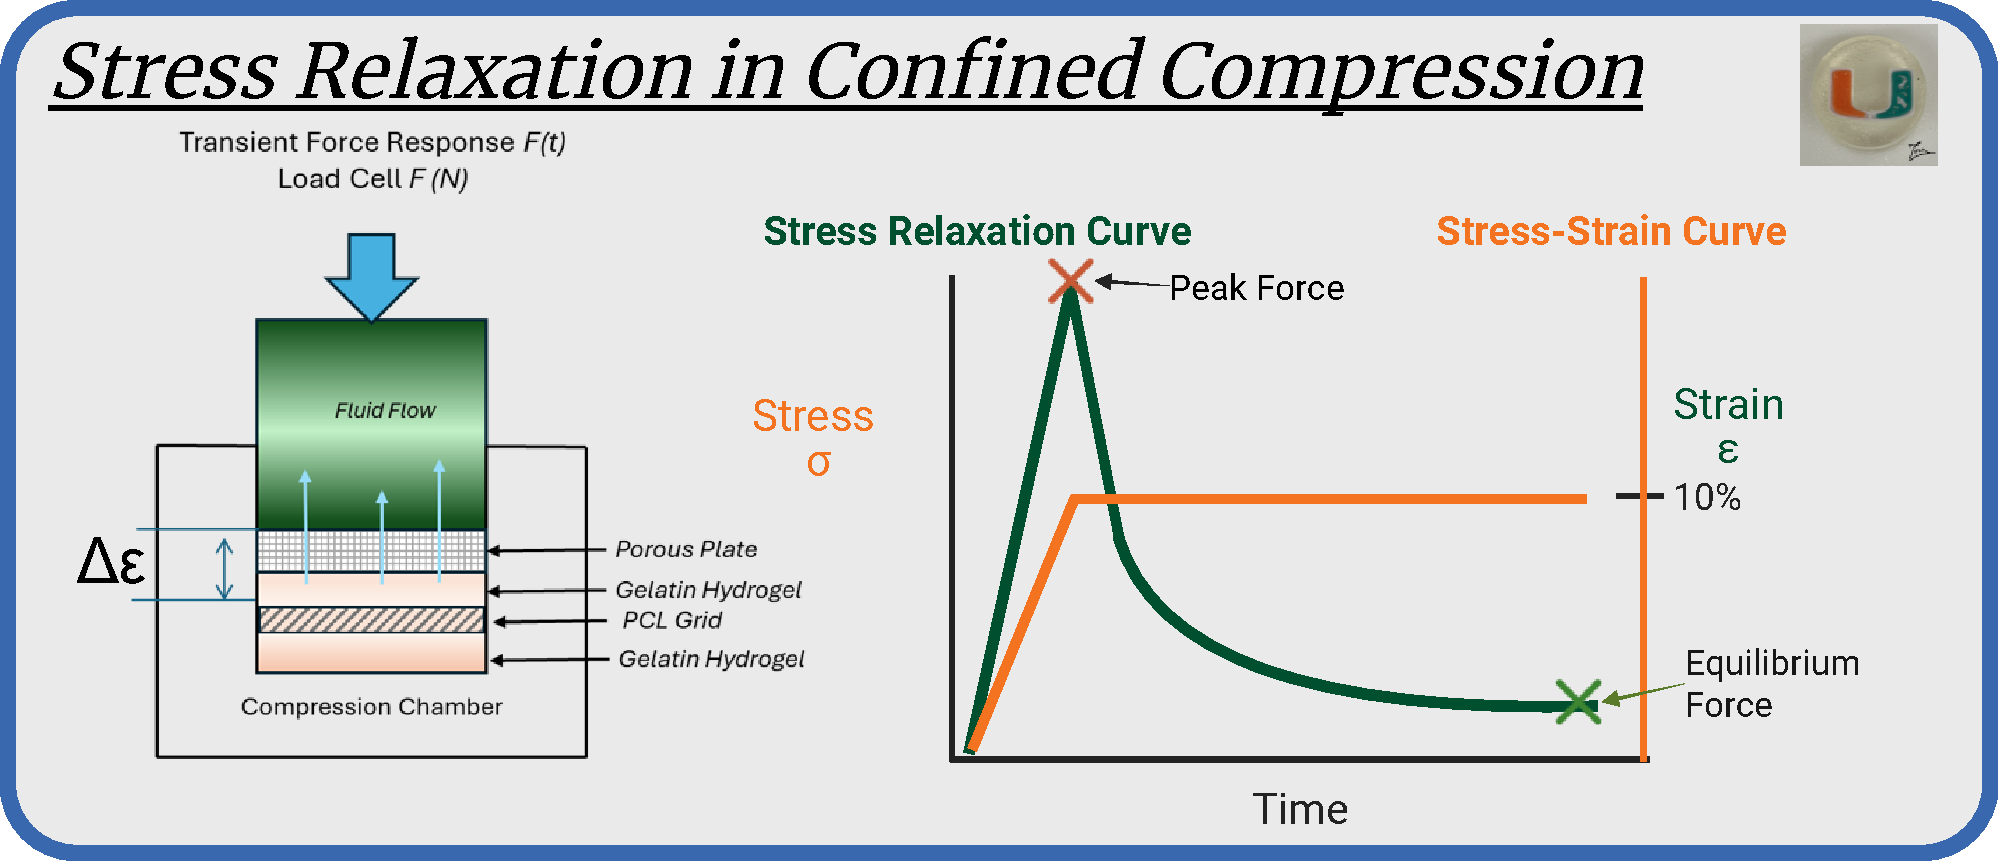
\includegraphics[width=1\linewidth]{figures/chapter 3/ch3_CCstressrelaxation.pdf}
    \caption[Schematic of stress relaxation in confined compression testing]{\textbf{Schematic of stress relaxation in confined compression testing.} The diagram (left) illustrates axial compression of a hydrogel scaffold within a confined chamber, forcing fluid flow through the porous platen. The accompanying plot (right) shows a typical stress relaxation curve, highlighting key parameters: peak force immediately after compression and equilibrium force following full relaxation at 10\% strain.}
    \label{fig:ch3_CCstressrelaxation}
\end{figure}

Stress relaxation testing provides critical insight into the viscoelastic and poroelastic behavior of hydrogels under confined conditions. After an initial rapid axial compression to a set strain (typically 10\%), the hydrogel is held at constant strain while the force response decays over time as fluid redistributes through the porous platen. This decay curve allows extraction of key mechanical parameters such as peak stress, equilibrium stress, and characteristic relaxation times. Confined compression stress relaxation is particularly relevant for simulating the in situ loading environment of the meniscus, where compressive forces act within a constrained anatomical space and fluid flow predominantly occurs axially.

\subsection{Testing Challenges and \protect\\ Boundary Condition Limitations}

While these models provide a clear theoretical basis, their assumptions are difficult to uphold in practice, leading to common testing challenges:

\textbf{1. Alignment and Edge Effects:}  
Even minor misalignment between compression platens and the sample surface introduces edge effects and non-uniform loading, violating the uniform axial stress assumption critical to both unconfined and confined models.

\textbf{2. Frictional Interactions:}  
In confined compression, friction between the hydrogel and chamber walls creates shear stresses and restricts fluid movement, breaching the assumption of frictionless radial boundaries. This skews both the stress field and pore pressure distribution.

\textbf{3. Pore Design Issues:}  
Non-uniform pore distribution in porous platens can cause irregular drainage paths, violating the boundary condition of uniform axial drainage, and resulting in heterogeneous stress relaxation behavior.

\textbf{4. Environmental Factors:}  
Sample dehydration, due to inadequate environmental control, alters hydration-dependent mechanical properties, invalidating the equilibrium assumptions embedded in the theoretical models.

\textbf{5. Visualization and Verification:}  
Opaque chambers prevent real-time verification of proper placement and deformation, increasing the risk of artifacts that are undetected until post hoc analysis.

\begin{figure}[H]
    \centering
    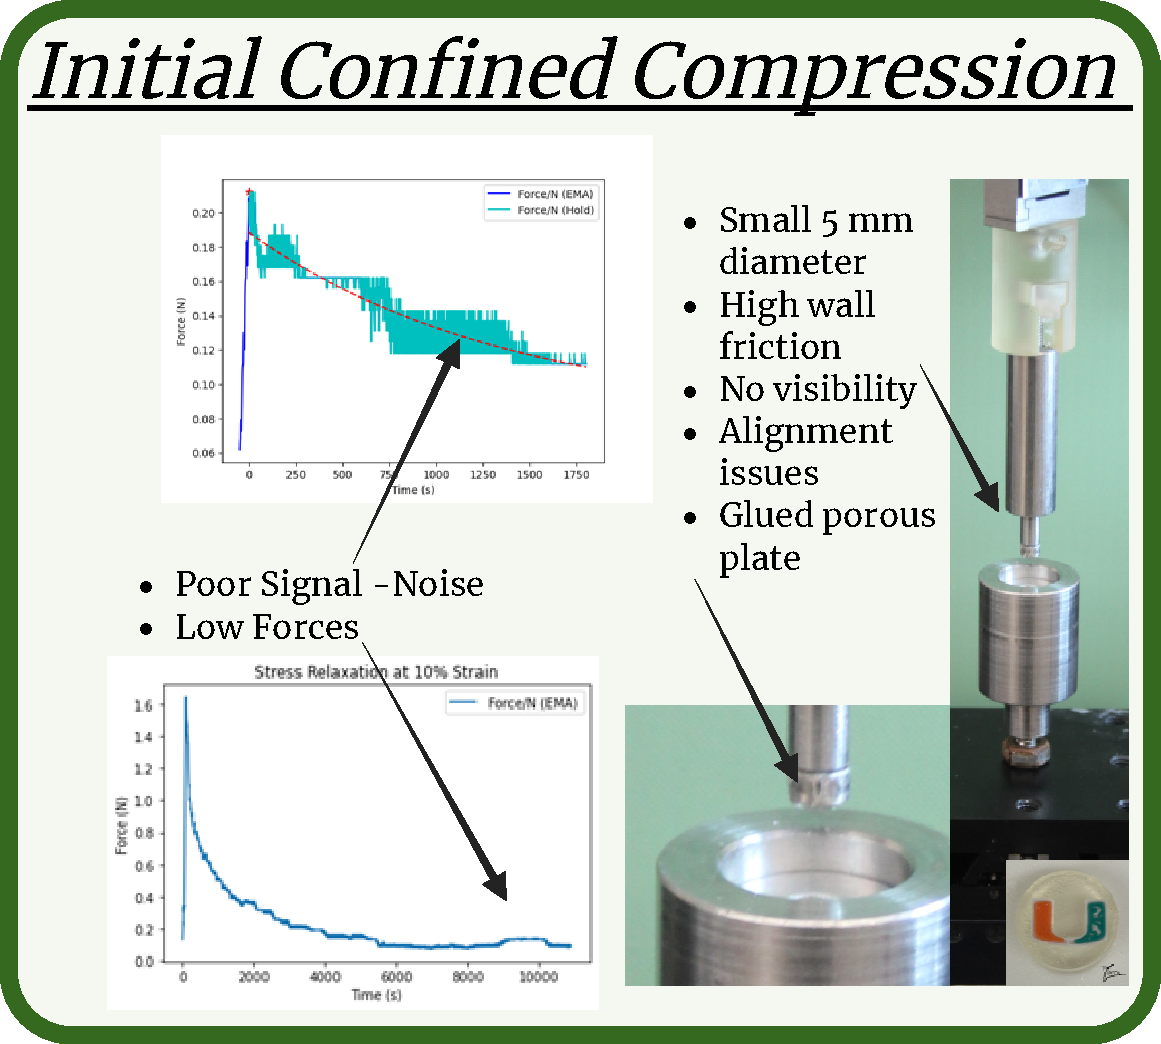
\includegraphics[width=1\linewidth]{figures/chapter 3/ch3_initialCC.pdf}
    \caption[Initial confined compression testing setup and limitations.]{\textbf{Initial confined compression testing setup and limitations.} The 5 mm diameter chamber (right) presented significant challenges, including high wall friction, a glued porous plate, and lack of visibility, all of which complicated alignment, cleaning, and accurate force measurements. Force–time plots (left) illustrate low-force detection and noisy signal output, highlighting the need for a redesigned testing platform. }
    \label{fig:ch3_initialCC}
\end{figure}

\section{"Augmentation" in Confined Compression Testing}

These challenges underscored the need for a customized testing system explicitly designed to uphold theoretical boundary conditions. Leveraging additive manufacturing allowed for rapid prototyping of a transparent, rigid, and precisely aligned confined compression chamber. Key design features included:

\begin{itemize}
    \item Increased sample surface area to enhance force detection and improve signal resolution
    \item High-precision alignment fixtures to minimize edge effects
    \item Smooth, rigid walls to maintain strict confinement
    \item Optimized porous platen design for uniform fluid drainage
    \item Transparent materials to allow real-time observation
    \item Integrated hydration control to preserve sample integrity throughout testing
\end{itemize}

This approach provided a robust framework for accurate poroviscoelastic characterization, bridging the gap between theoretical modeling and experimental practice.

\subsection{Data Analysis and Signal Processing}

The analysis of compression testing data requires sophisticated signal processing techniques to ensure accurate interpretation of material properties. Raw data from compression tests often contains various forms of noise and artifacts that must be carefully addressed through systematic processing approaches.

A custom Python script was also developed to streamline data processing and enhance reproducibility (see Appendix~\ref{appendix:data_analysis_script}). The script automates key steps including batch processing of CSV files, extraction of force data for specific strain regions (5\%, 10\%, 20\%), and application of signal smoothing using an Exponential Moving Average (EMA). It fits exponential decay curves to the force-relaxation data, extracting parameters such as peak force, equilibrium force, and the time constant. Additional features include Fourier analysis for noise characterization, automated plot generation, and compilation of mechanical parameters into an Excel summary file, ensuring both precision and efficiency in data analysis. 

\begin{figure}[H]
    \centering
    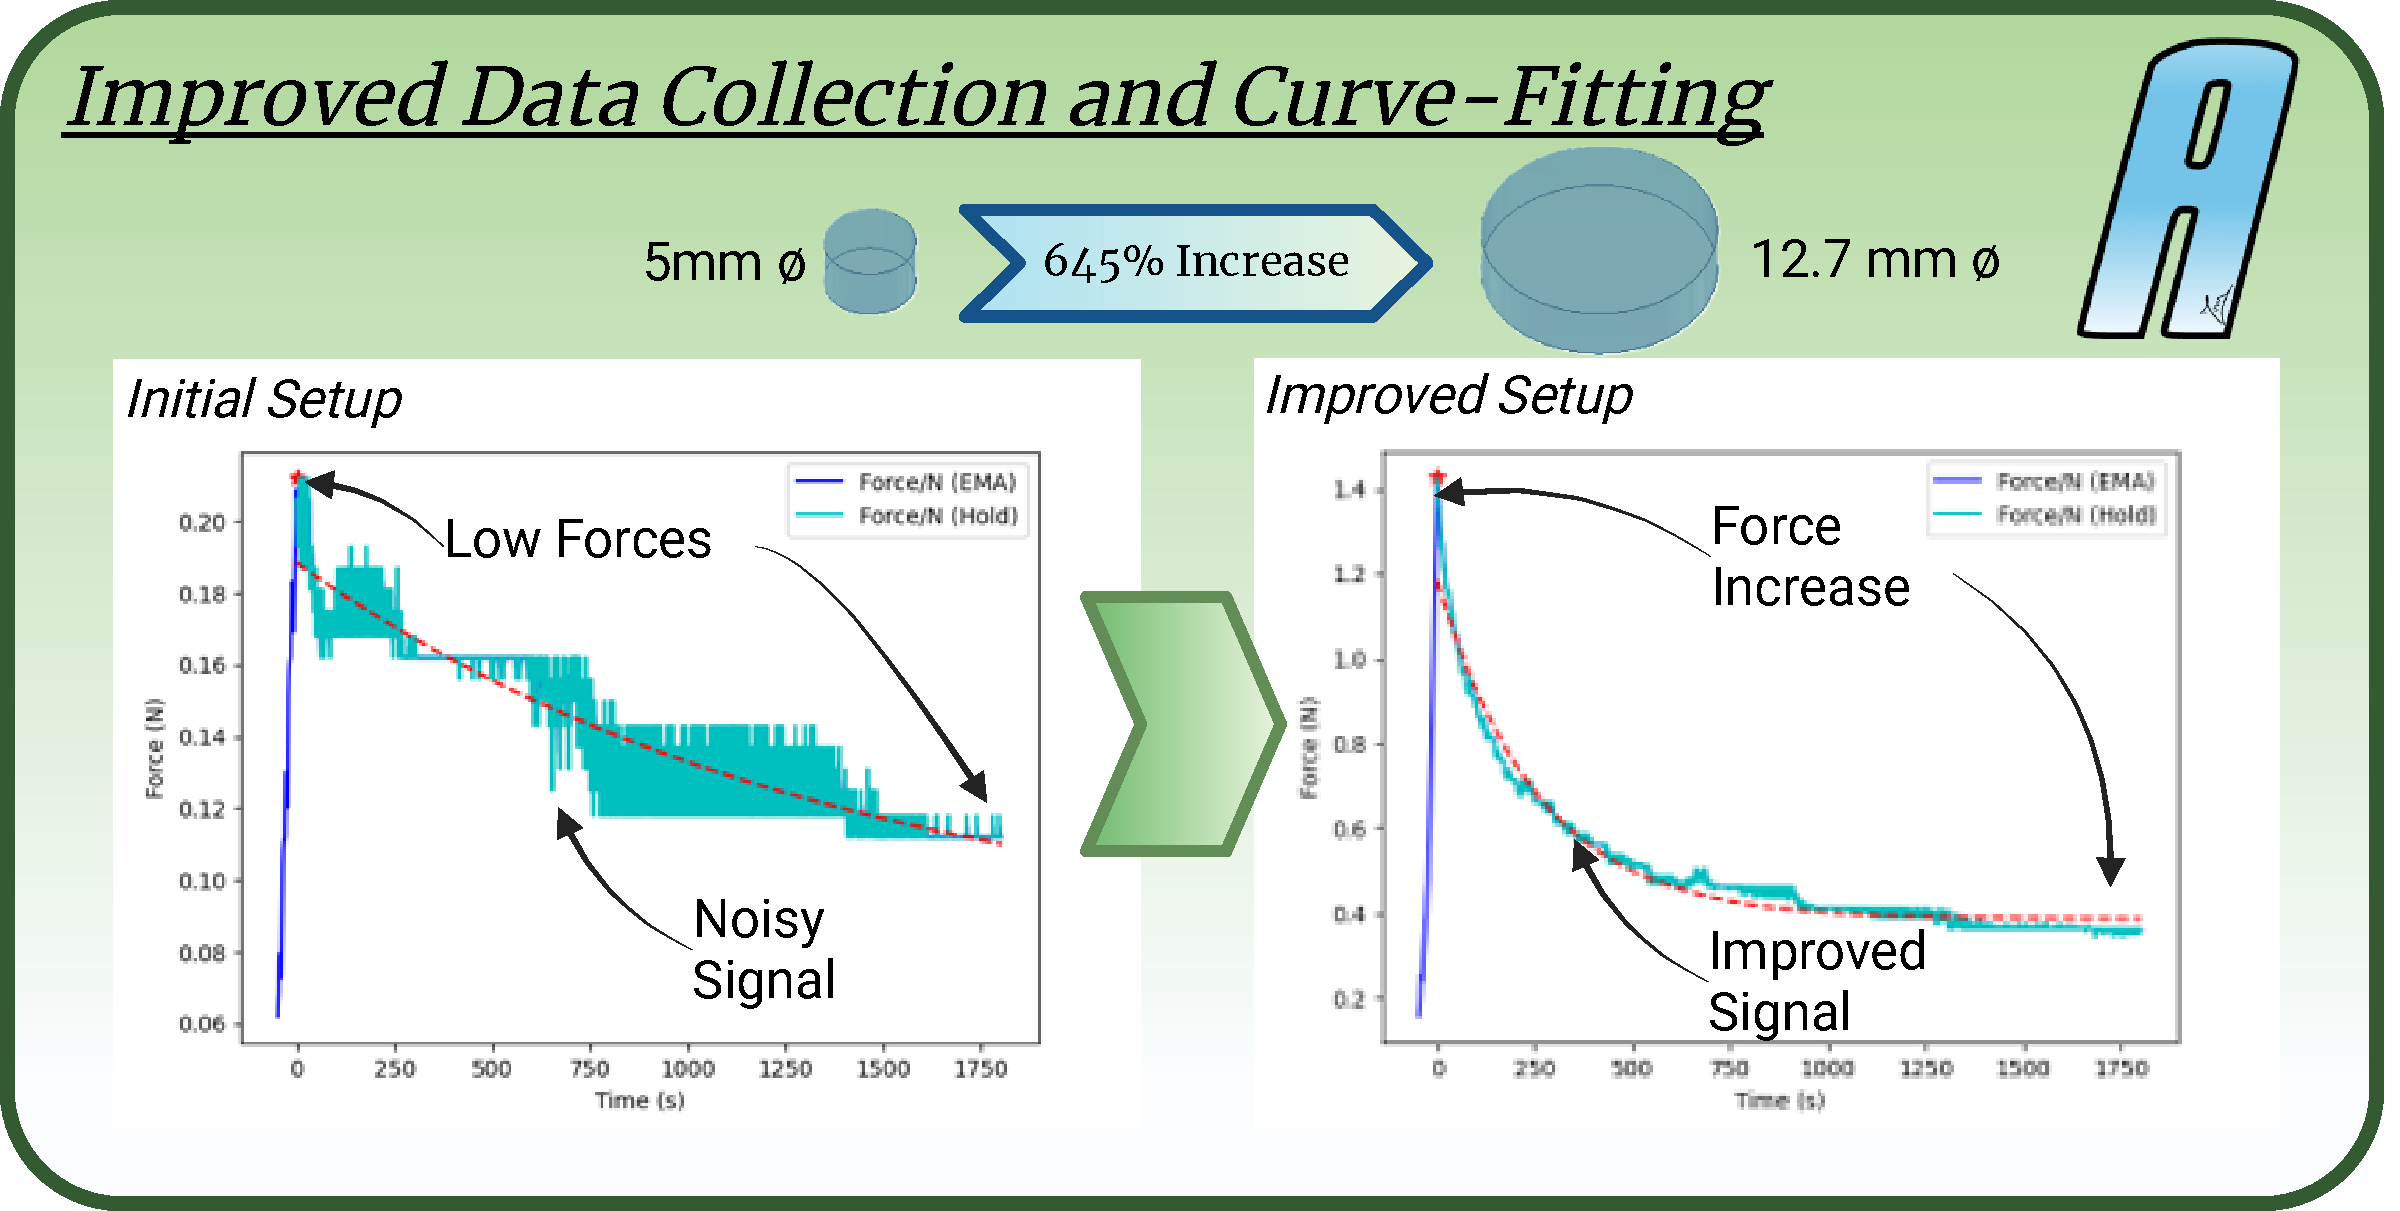
\includegraphics[width=1\linewidth]{figures/chapter 3/ch3_signalAug.pdf}
    \caption[Improved data collection and curve-fitting in confined compression testing]{\textbf{Improved data collection and curve-fitting in confined compression testing.} Comparison between the initial setup (left), featuring a 5 mm diameter chamber, and the improved setup (right) with a 12.7 mm diameter chamber. The larger chamber resulted in a 645\% increase in cross-sectional area, enabling higher force readings and significantly reducing signal noise. Enhanced signal quality and force detection improved the reliability of stress-relaxation data and curve-fitting accuracy. }
    \label{fig:ch3_signalAug}
\end{figure}

Data normalization is a critical step that enables meaningful comparisons between different samples and testing conditions. This process typically involves normalizing stress values to account for variations in initial sample dimensions, adjusting time scales to compensate for differences in loading rates, and standardizing strain measurements relative to the initial sample height. Such normalization ensures that the intrinsic material properties can be evaluated independently of variations in sample geometry or specific test parameters.

For stress relaxation data, experimental results are fitted to theoretical models such as:

$$\sigma(t) = \sigma_{\infty} + (\sigma_0 - \sigma_{\infty})e^{-t/\tau}$$

where $\sigma_{\infty}$ represents the equilibrium stress, $\sigma_0$ is the peak stress, and $\tau$ is the characteristic relaxation time.

\subsection{Material Property Extraction}

The extraction of material properties from mechanical testing data requires consideration of underlying physical models that describe the poroviscoelastic behavior of hydrated biomaterials~\cite{ateshian1997finitedeformation}. Two key mechanical parameters are typically derived from stress-relaxation testing:

\textbf{Peak modulus} is calculated from the initial loading response, representing the instantaneous mechanical resistance of the material to applied deformation~\cite{boschetti2004biomechanicalproperties}. This parameter reflects the combined contribution of both solid matrix stiffness and fluid pressurization effects~\cite{ateshian1997finitedeformation}.

\textbf{Equilibrium modulus} is derived from the steady-state stress after complete relaxation, representing the long-term mechanical behavior when fluid flow has ceased and only the solid matrix contributes to load bearing~\cite{buschmannconfinedcompression,koch2022mechanicalproperties}.

\textbf{Permeability} characterizes the fluid transport properties of the material and can be calculated using different approaches depending on the testing configuration~\cite{mansour1976permeabilityarticular,loverde2024compressioncycling, nakagawa2019longtermevaluation}:

For confined compression testing:
\begin{equation}
k = \frac{h^2 \mu}{E \tau}
\end{equation}

For unconfined compression testing:
\begin{equation}
k = \frac{a^2 \mu}{E \tau}
\end{equation}

where $h$ is sample thickness, $a$ is sample radius, $\mu$ is fluid viscosity, $E$ is the appropriate modulus (peak or equilibrium), and $\tau$ is the characteristic relaxation time constant~\cite{ateshian1997finitedeformation, boschetti2004biomechanicalproperties}.

These material properties provide essential information for characterizing the mechanical and transport behavior of hydrogel scaffolds, enabling comparison with native tissue properties and optimization of scaffold design parameters~\cite{morejon2020compressiveproperties}.

\subsection{Common Issues and Solutions}

Several challenges commonly arise during compression testing of hydrogels, which can compromise data quality if not properly addressed. Key issues include non-linear initial responses, signal noise, and baseline drift.

\textbf{Non-linear Initial Response.} An unexpected non-linear region at the beginning of the stress--strain curve often indicates poor platen-to-sample contact, stemming from either misalignment or uneven sample surfaces. This can be resolved by implementing rigorous alignment verification protocols and standardizing sample preparation methods.

\textbf{Signal Noise.} Data can be contaminated by environmental vibrations, electrical interference with measurement instruments, or inaccuracies in the load cell. To mitigate this, testing should be conducted when building vibrations are minimal, and force readings must be verified to be within the expected range of the load cell.

\textbf{Baseline Drift.} During long-term experiments, gradual baseline shifts may occur due to progressive sample dehydration or temperature fluctuations affecting both the sample and equipment. Maintaining strict environmental controls throughout testing is critical to prevent such artifacts.

A systematic approach to quality control, including regular calibration and protocol validation, is essential for ensuring reliable and reproducible mechanical characterization results.

\section{Design and Additive Fabrication of the Confined Compression Apparatus}

To address the limitations of conventional confined compression systems, we developed a novel, custom testing apparatus tailored specifically for soft hydrogel characterization. The design process focused on enhancing measurement precision, reproducibility, and physiological relevance, while overcoming challenges related to friction, visibility, and sample handling. Additive manufacturing, particularly stereolithography (SLA), provided the flexibility and precision required to fabricate specialized components with optimal properties.

Recent developments in 3D bioprinting have expanded possibilities for creating complex tissue architectures~\cite{klarmann20243dbioprinting}. These technologies enable precise control over scaffold geometry and material distribution. The integration of digital light processing techniques has further enhanced the resolution and accuracy of additively manufactured components~\cite{hong2020digitallight}, enabling testing apparatus features impossible through traditional manufacturing.

Through iterative design cycles, we refined the chamber geometry and material selection to balance mechanical strength with visual accessibility. The final apparatus featured a transparent compression chamber fabricated using high-resolution digital light synthesis (DLS) 3D printing with Loctite Henkel 405 Clear Resin (Young's Modulus $\sim$1350~MPa), selected for its rigidity and optical clarity.

Finite element analysis confirmed negligible chamber deformation ($1.4~\mu\mathrm{m}$) under maximum expected loading (20~N). To improve force sensitivity, we scaled the chamber to hold 12.7~mm diameter specimens—resulting in a 645\% increase in surface area compared to conventional 5~mm chambers—while maintaining compatibility with existing mold designs.

\subsection{Additive Fabrication and Post-Processing}

The compression chamber and platen components were fabricated using a Carbon3D M1 DLS SLA printer at 50~µm Z-layer resolution. Throughout the fabrication process, part orientation and tolerances were optimized to maximize optical transparency of the compression chamber, dimensional accuracy within the XY plane, and fit and function of critical design features. The selection of the Carbon3D M1 printer was driven by its ability to produce parts with exceptional surface finish and dimensional precision, essential for achieving the tight tolerances required for accurate mechanical testing.

The fabrication process involved careful consideration of print orientation to minimize support structures while maximizing the optical clarity of critical viewing surfaces. Parts were oriented to ensure that the primary viewing windows of the compression chamber faced upward during printing, reducing the need for post-processing on these critical surfaces. Additionally, the build orientation was optimized to minimize layer lines that could interfere with visual monitoring during testing procedures.

The impact of manufacturing processes on material properties has been extensively studied~\cite{maldonado-codina2004impactmanufacturing,demulder2009anisotropicporous,fernandes2021mechanicallyrobust,davis2004polymerchemistry}, revealing how processing parameters can significantly influence the mechanical and optical characteristics of additively manufactured components. Understanding these relationships is essential for optimizing the fabrication process to achieve the desired balance of mechanical strength, optical clarity, and dimensional accuracy required for precise mechanical testing applications.

\begin{figure}[H]
    \centering
    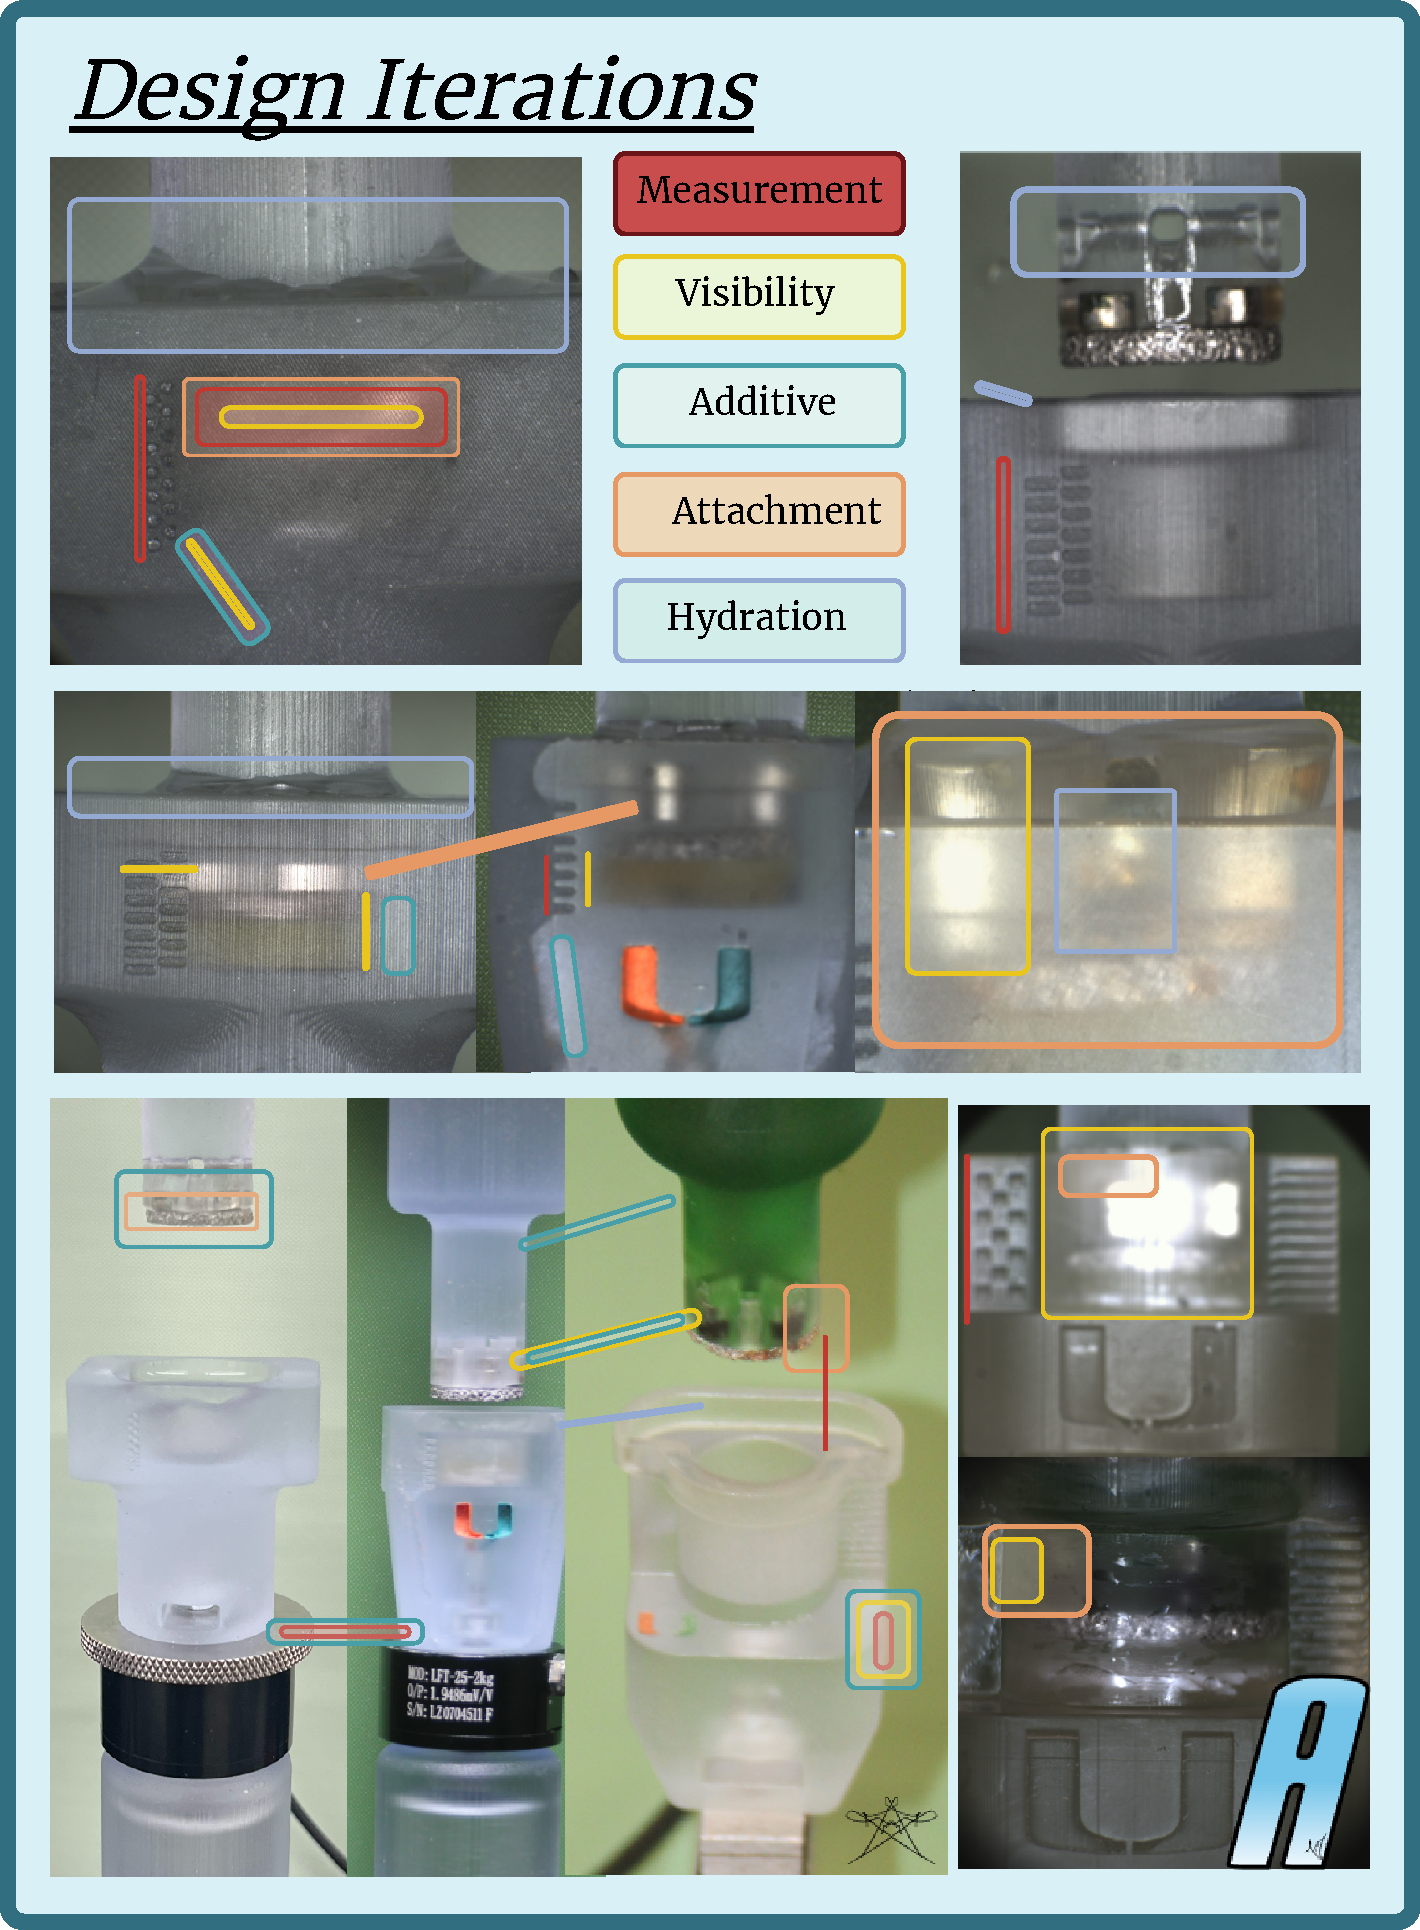
\includegraphics[width=0.92\linewidth]{figures/chapter 3/ch3_iterations.pdf}
    \caption[Iterative design development with color-coded highlights and feature linkages]{\textbf{Iterative design development with color-coded highlights and feature linkages.} This composite image traces the progressive refinement of the confined compression testing chamber, with inset windows highlighting specific changes or challenges across five key design categories: Measurement (red), Visibility (yellow), Attachment (orange), Additive (blue), and Hydration (teal). }
    \label{fig:ch3_iterations}
\end{figure}

\subsection{Iterative Design Development}

The iterative design process balanced mechanical performance, usability, and manufacturability through multiple cycles of refinement. Color-coded highlights and connecting lines in the figure demonstrate the evolution and interdependence of key features, where improvements in one area (like magnetic attachments reducing friction) often created new challenges (such as visibility obstruction and corrosion) that required further optimization.

\begin{itemize}
    \item \textbf{Measurement (red):} Design elements aimed at reducing friction and improving load cell accuracy, such as interface refinements and integrated scale bars to enable more precise hydrogel/composite measurement.
    \item \textbf{Visibility (yellow):} Modifications to improve optical clarity, facilitating real-time monitoring of sample placement, defect detection, and platen contact verification.
    \item \textbf{Attachment (orange):} Introduction of magnetic suspension systems to minimize friction and enhance measurement precision, balanced against challenges of visibility obstruction and corrosion in hydrated environments.
    \item \textbf{Additive (blue):} Enhancements linked to 3D printing strategies, including geometry optimization and print orientation (often indicated by angled lines), to improve surface smoothness, transparency, and dimensional accuracy.
    \item \textbf{Hydration (teal):} Features designed to maintain sample hydration and integrity, which also influenced other components, such as contributing to rust formation in metallic attachments.
\end{itemize}

This integrated approach ensured that each design iteration not only solved isolated issues but also accounted for broader system interactions, reinforcing the need for holistic optimization across all design domains.



\begin{figure}[H]
    \centering
    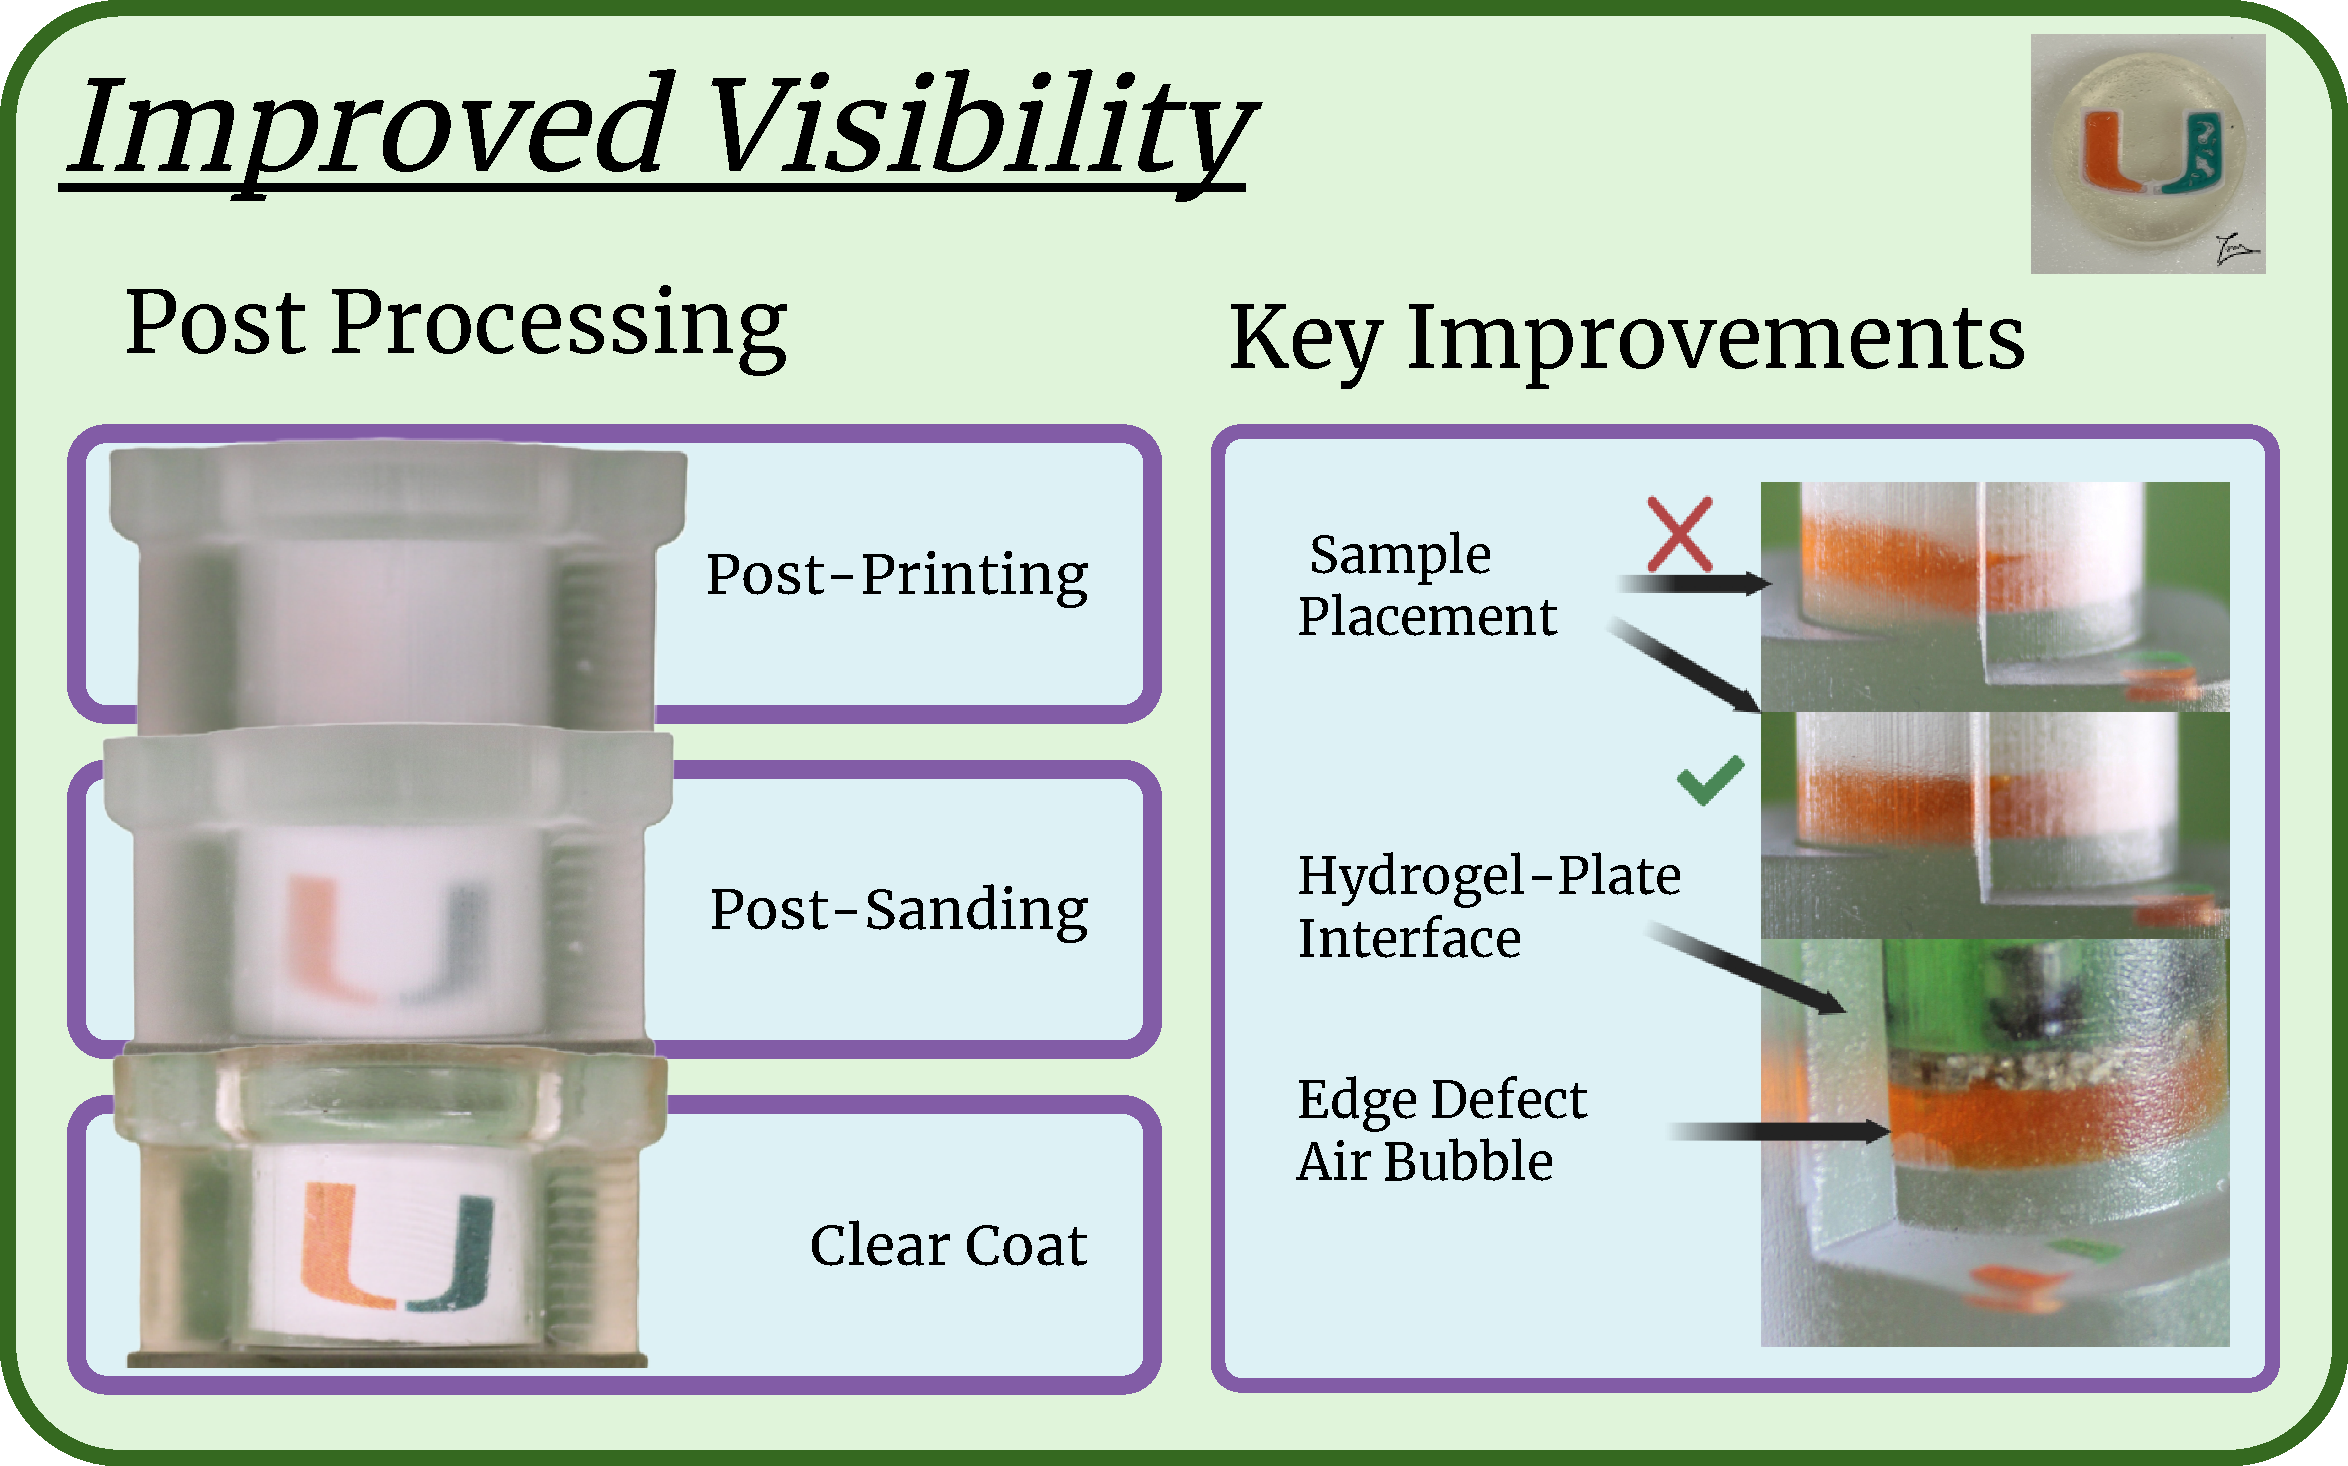
\includegraphics[width=1\linewidth]{figures/chapter 3/ch3_visibility.pdf}
    \caption[Enhanced chamber visibility]{\textbf{Enhanced chamber visibility.} Progressive improvement in chamber transparency through post-processing steps (left) enables improved sample monitoring and defect detection (right).}
    \label{fig:ch3_visibility}\end{figure}

To enhance visibility, we developed a streamlined post-processing workflow involving wet sanding (400 to 2000 grit) and clear coating. This progression significantly improved optical clarity for real-time monitoring—a critical improvement over traditional opaque chambers. Two layers of clear coat provided a mirror-like finish while protecting against moisture damage. The resulting components achieved optical clarity comparable to commercial glass while maintaining dimensional precision.

The additive manufacturing approach enabled complex internal geometries impossible with traditional machining. Components were fabricated as single units, eliminating assembly needs and reducing error sources. Rapid prototyping capabilities facilitated quick design iteration and optimization.

\clearpage
\subsection{Key Design Innovations and Takeaways}

The custom confined compression system, developed using SLA printing, introduced several critical innovations that enhanced testing accuracy for soft, hydrated biomaterials:

\begin{itemize}
    \item \textbf{Transparent, Modular Design:} The additively manufactured transparent chamber enabled real-time visual monitoring and consistent confinement geometry. The modular construction facilitated rapid disassembly and cleaning between tests.
    
    \item \textbf{Magnetically Suspended Platen:} The magnetic suspension system minimized friction between components and self-centered during sample engagement, eliminating mechanical bearings that could introduce measurement artifacts.
    
    \item \textbf{Optical Access:} Integrated macro-imaging capabilities ensured precise platen-to-sample alignment, reducing measurement artifacts common in conventional opaque chambers.
    
    \item \textbf{Optimized Force Detection:} A 20~N high-resolution load cell improved force detection by 200--1600\% over conventional setups, enabling detection of subtle mechanical differences between hydrogel formulations.
    
    \item \textbf{Environmental Control:} The integrated system allowed continuous PBS rehydration during extended tests to maintain sample integrity.
\end{itemize}

These features significantly improved measurement precision, reproducibility, and physiological relevance. The integration of additive manufacturing with precision mechanical testing demonstrated how rapid prototyping can accelerate biomaterials research through customized instrumentation development. The substantial improvements in measurement sensitivity have enabled more reliable differentiation between mechanically distinct hydrogel formulations—critical for biomaterial development where subtle mechanical differences can significantly impact functional outcomes.

\clearpage
\section{Assembly, Alignment, and Sample Handling}

Having established the design and fabrication approach for the confined compression apparatus, precise assembly, alignment protocols, and standardized sample handling procedures were developed to ensure consistent and reliable mechanical testing results. These operational protocols were critical for maximizing the benefits of the improved hardware design.

Ensuring precise alignment between the compression platen and the hydrogel sample was critical for minimizing measurement artifacts and maintaining consistent testing conditions. Prior to each test, the compressing plug was carefully aligned using an adjustable XY centering stage. Alignment was visually guided through macro camera imaging, which allowed for fine positional adjustments and ensured that the plug was centered over the specimen without tilting or lateral offset.

Further validation of alignment was achieved through the use of a magnetically suspended porous platen, which ensured consistent contact with minimal frictional resistance. Magnetic plate attachment stability was checked to confirm that no lateral shear or misalignment forces were introduced during initial platen engagement. Prior to mechanical loading, the sample position within the chamber and the initial contact with the porous platen were visually confirmed through the transparent chamber walls.

\subsection{Sample Preparation and Handling Protocols}

Careful sample preparation and handling were essential for obtaining reliable mechanical testing results. Cylindrical hydrogel samples were prepared using custom PTFE molds engineered to produce specimens of consistent diameter and height. The molds were precision-machined with polished surfaces to minimize sample adhesion and ensure clean removal. Prior to testing, samples were equilibrated in phosphate-buffered saline (PBS) at room temperature for at least a full day to achieve complete hydration and dimensional stability.

Loading and positioning of samples within the testing chamber followed a standardized protocol:
\begin{itemize}
    \item The hydrogel sample was carefully transferred using wide-tip forceps to minimize damage, gripping only the outer edges
    \item Visual inspection through the transparent chamber confirmed proper sample positioning and ensured no trapped air bubbles
    \item The magnetically attached porous platen was gently lowered onto the sample surface at a slow, controlled rate
    \item The chamber was filled with additional PBS to maintain full hydration throughout testing, with careful attention to avoid disturbing the sample
    \item Initial contact force was monitored to ensure minimal preload during setup
    \item Testing commenced only after visual confirmation of proper alignment and sample placement
\end{itemize}

Between tests, the chamber and platens were thoroughly cleaned with deionized water and dried to prevent cross-contamination. The magnetic attachment surfaces were inspected for debris that could affect alignment. Regular calibration checks were performed to maintain measurement accuracy. This comprehensive and standardized approach to sample handling significantly improved test-to-test reproducibility and minimized operator-dependent variability in mechanical measurements, achieving excellent consistency across multiple testing sessions.

\begin{figure}[H]
    \centering
    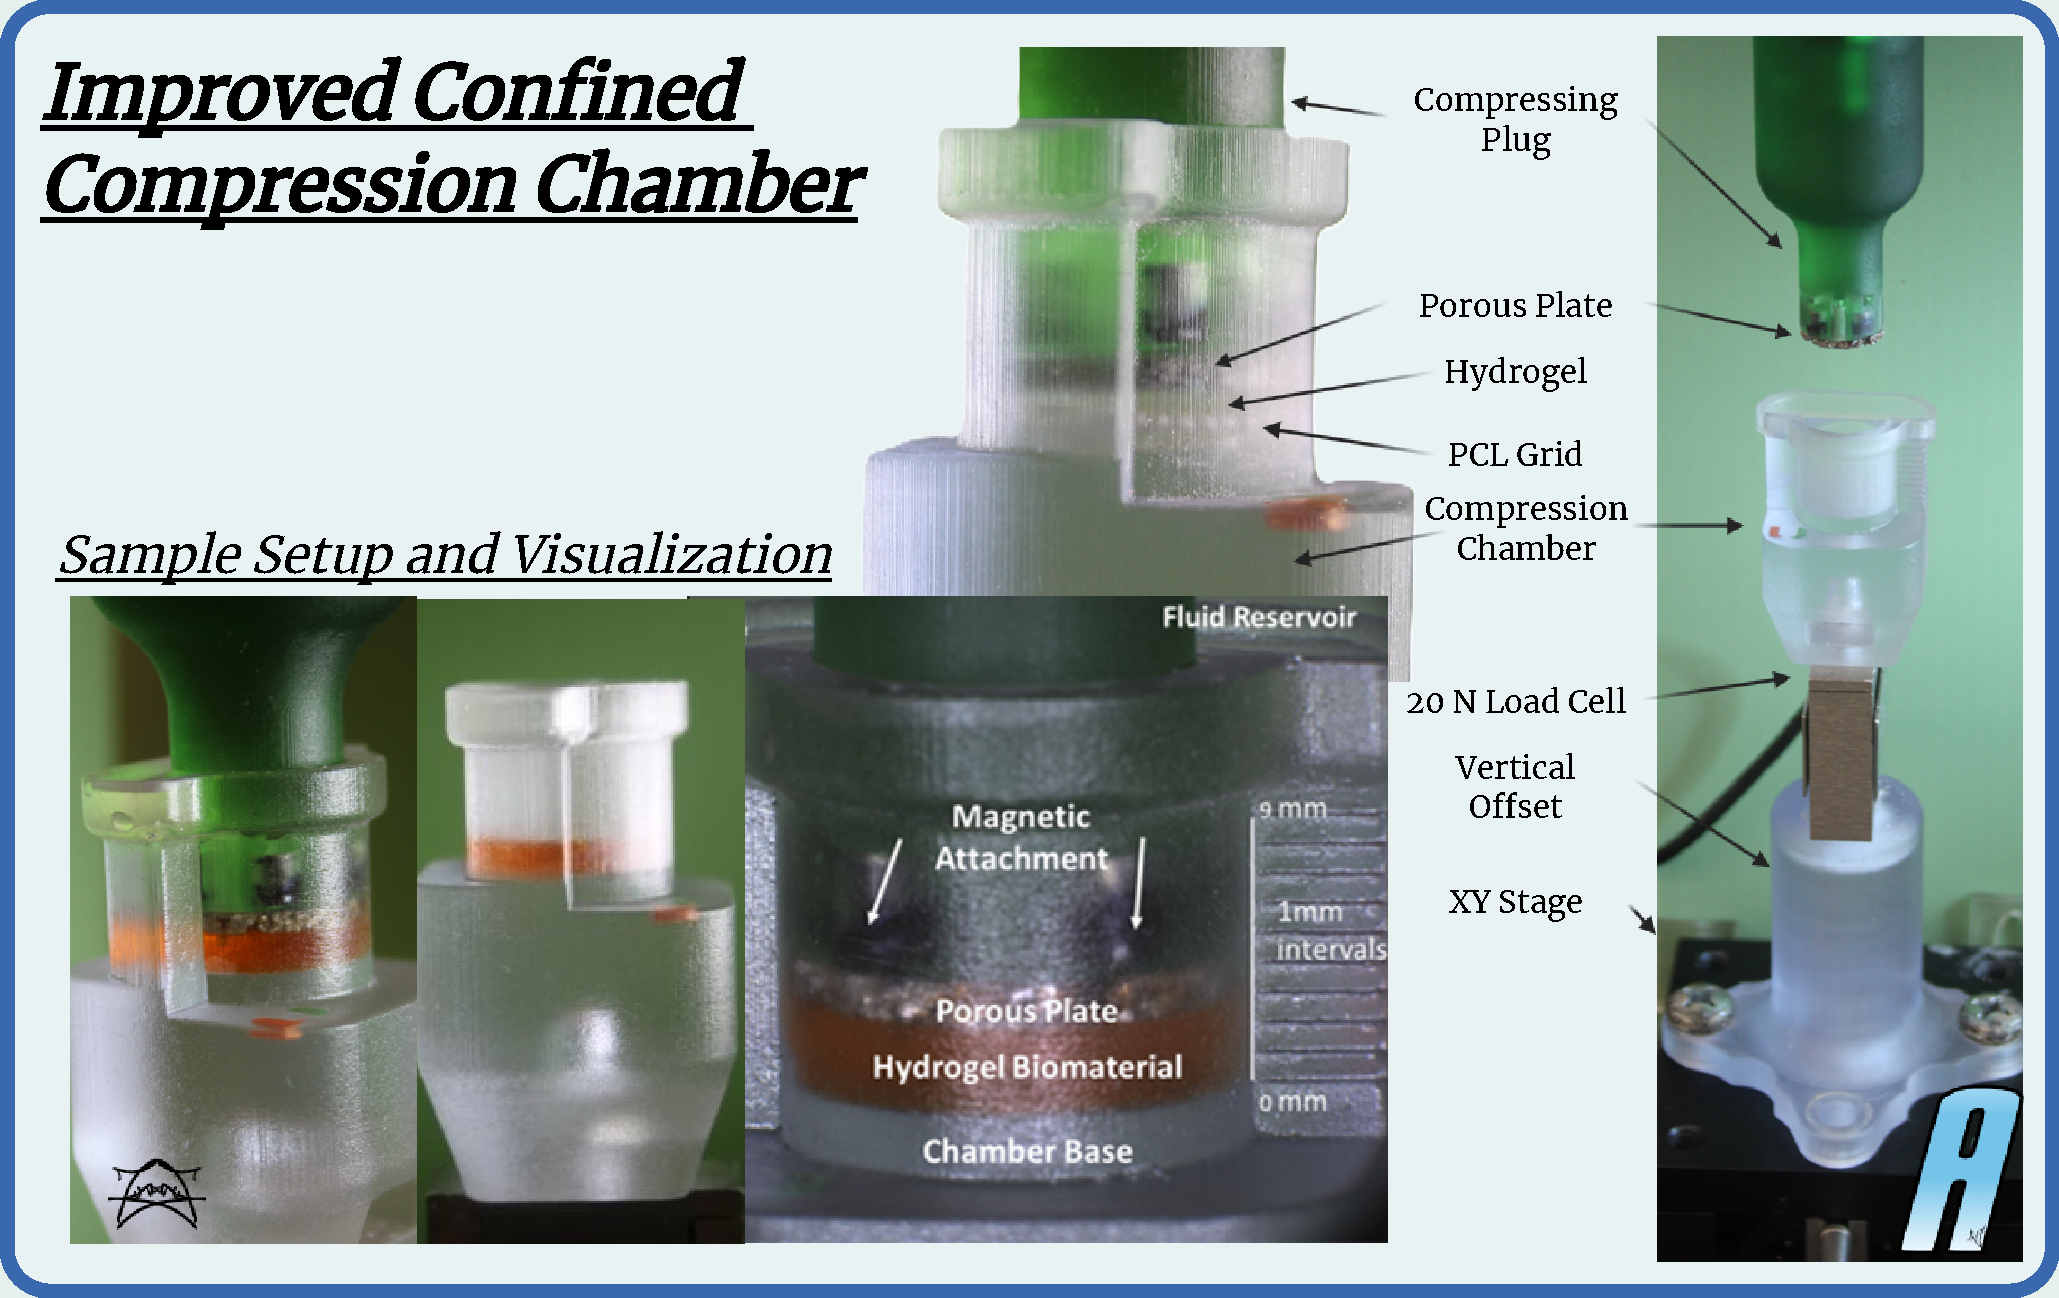
\includegraphics[width=0.9\textwidth]{figures/chapter 3/ch3_finalCC.pdf}
    \caption[Improved confined compression chamber with enhanced sample setup and visualization]{\textbf{Improved confined compression chamber with enhanced sample setup and visualization.} The diagram highlights key components of the custom testing system, including the compression plug, porous plate, hydrogel sample, PCL grid, and chamber base. Insets illustrate sample placement, magnetic attachment of the porous plate, and real-time visualization of the hydrogel–platen interface. The full assembly, shown mounted with a 20 N load cell and XY stage, demonstrates the integrated system designed for precise alignment and controlled mechanical testing.}
    \label{fig:Ch3_Assembly}
\end{figure}

\clearpage
\section{Validation of Improved Testing Setup:\protect\\Initial vs. Improved Comparison}

To evaluate the performance improvements of the custom testing setup, two types of hydrogels were tested: gelatin A hydrogels with varying glutaraldehyde (GTA) crosslinking concentrations (0.5\% and 1.5\%) and agarose hydrogels at different concentrations (2\% and 4\% w/v) as control materials. These materials were selected to represent a range of mechanical properties relevant for meniscal tissue engineering applications, with gelatin A hydrogels being the primary material of interest and agarose serving as a well-characterized control.

The mechanical testing protocol was designed to evaluate both the instantaneous and time-dependent properties of the hydrogel formulations. Cylindrical samples (12.7 mm diameter) were subjected to confined compression testing using the custom apparatus. After a 0.15 N preload to ensure proper contact, samples were compressed to 10\% strain at a rate of 0.1\%/s (3.12 µm/s) while submerged in PBS at room temperature (22°C). The strain was held constant for 60 minutes while stress relaxation data was collected.

Force measurements were recorded at 1 Hz during both the ramp and hold phases using a 20N load cell. Key parameters extracted from the tests included:

\begin{itemize}
    \item \textbf{Peak Force} (\(F_{\text{peak}}\)): The maximum force recorded at the end of the loading phase when the target strain (10\%) was achieved.
    
    \item \textbf{Equilibrium Force} (\(F_{\text{eq}}\)): The force measured after stress relaxation plateaued, typically determined at the end of the 60-minute hold period.
    
    \item \textbf{Aggregate Modulus} (\(H_A\)): A measure of the material's compressive stiffness under confined conditions, calculated based on the equilibrium stress and applied strain.
\end{itemize}

\begin{equation}
    H_A = \frac{\sigma_{\text{eq}}}{\epsilon}
\end{equation}

where \(\sigma_{\text{eq}}\) is the equilibrium stress (equilibrium force divided by the initial cross-sectional area), and \(\epsilon\) is the applied strain (10\%).

\subsection{Experimental Design and Data Analysis}

Raw force-time data was processed using custom Python scripts to extract key mechanical parameters. Stress-time and stress-strain curves were generated using the initial cross-sectional area of the samples. Stress relaxation data was analyzed to determine the time-dependent decay characteristics, including relaxation time constants and equilibrium stress values.

Statistical analyses were performed using two-way ANOVA to assess the effects of material formulation and testing setup (Initial vs. Improved) on mechanical parameters. Post-hoc comparisons were conducted using Fisher's LSD test with a significance threshold of p<0.05.

\subsection{Performance Comparison: Initial vs. Improved Testing Apparatus}

To validate the performance and improvements of the novel confined compression apparatus, a direct comparison was conducted against a conventional confined compression setup. Testing was performed on identical hydrogel formulations using both systems, allowing for side-by-side assessment of measurement sensitivity, reproducibility, and physiologically relevant force detection.

\begin{figure}[H]
    \centering
    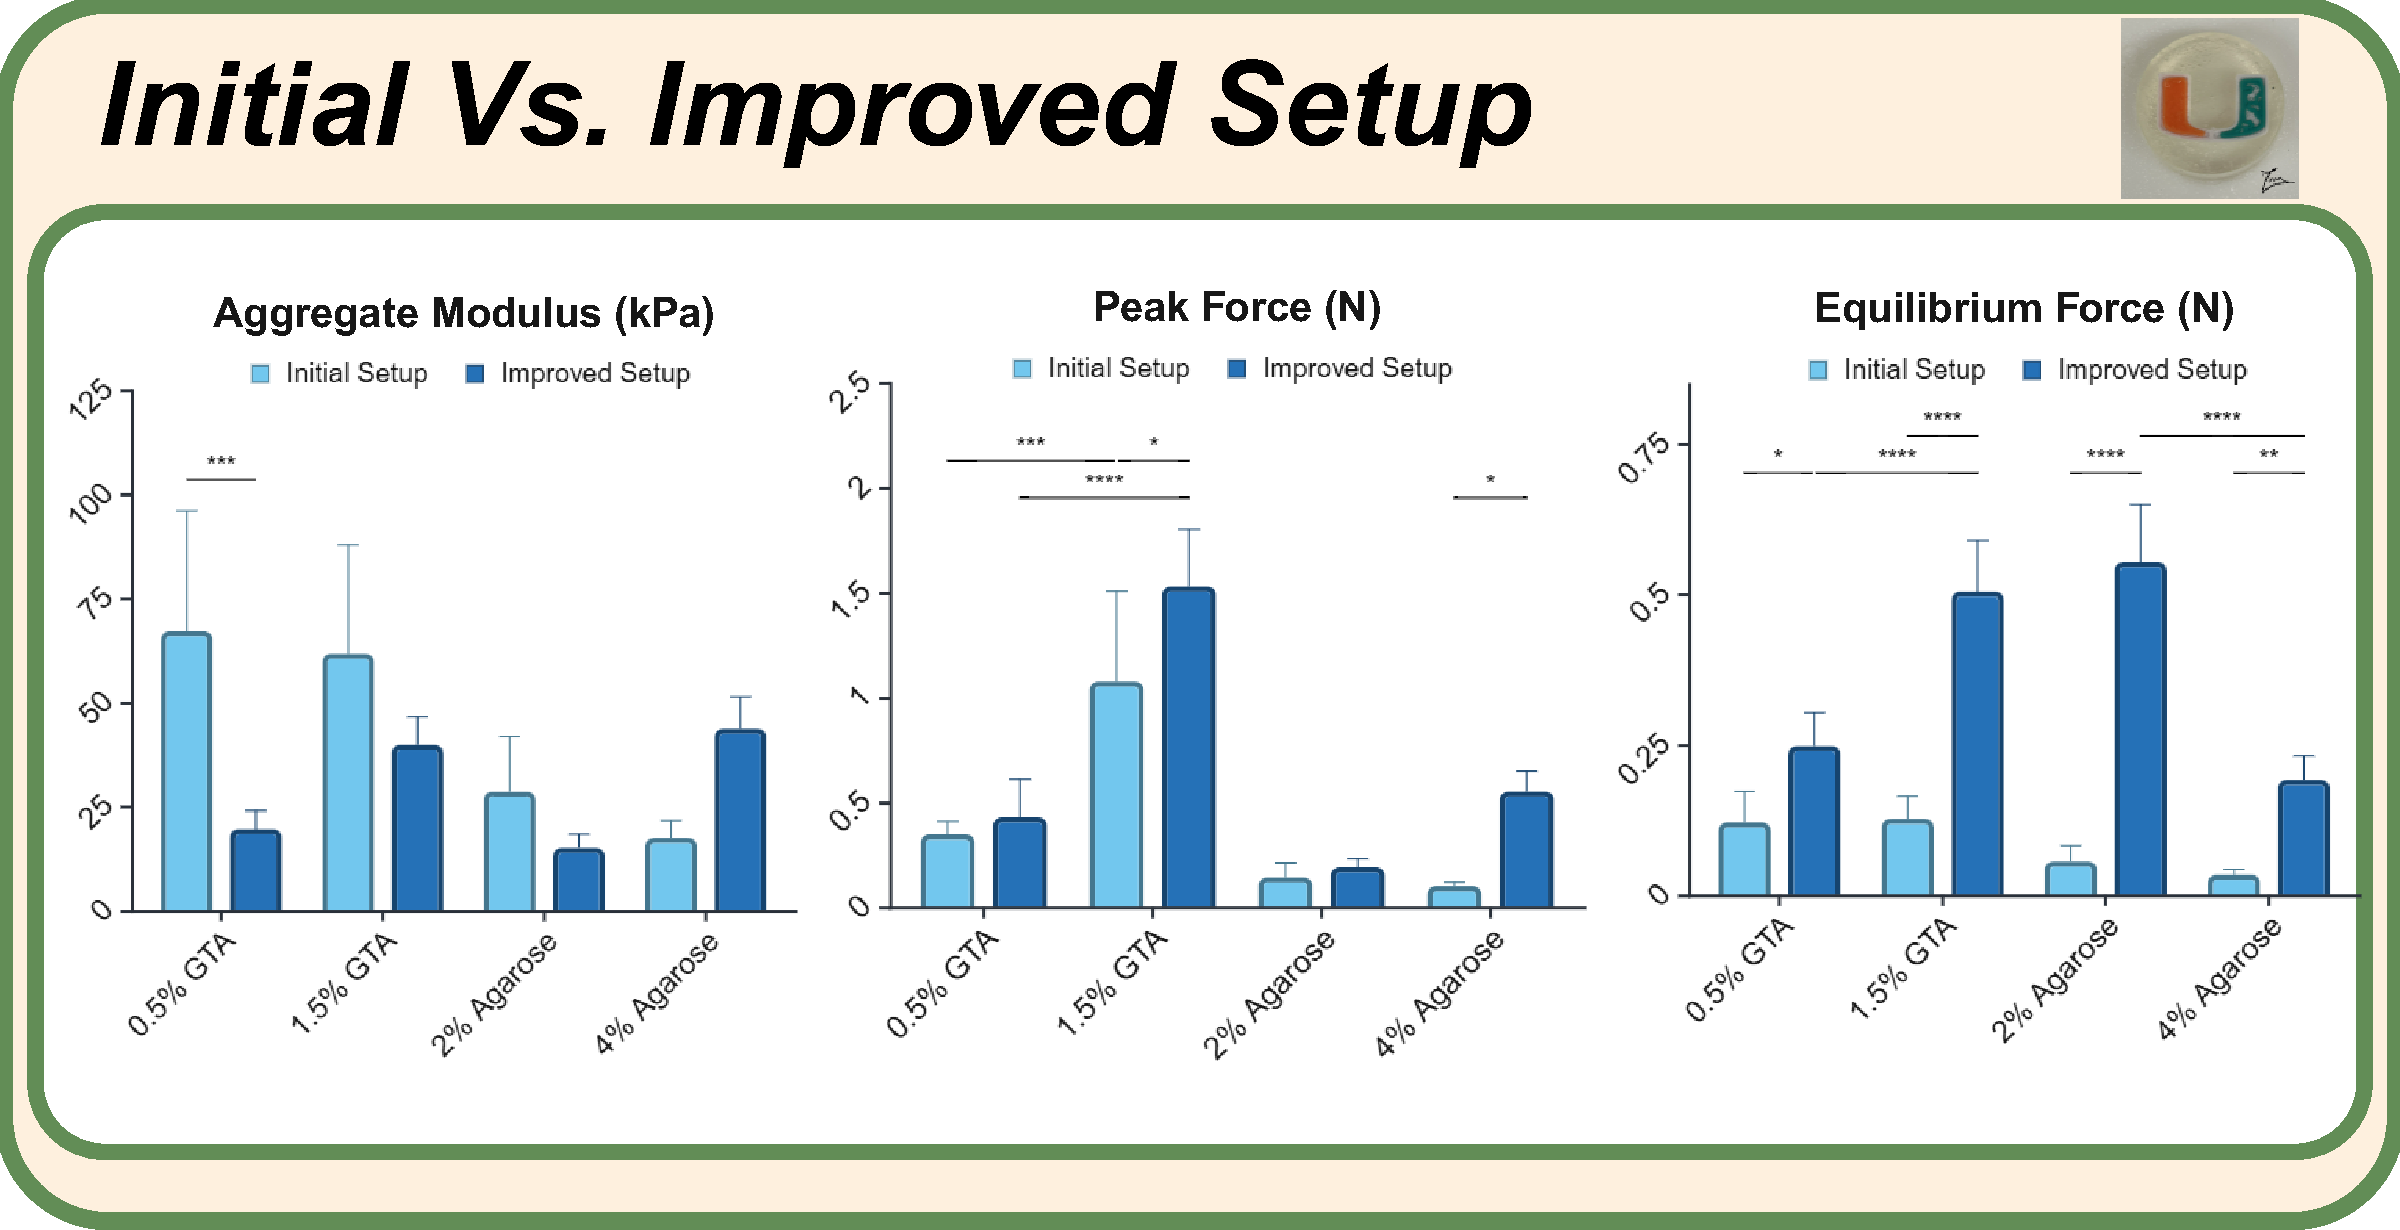
\includegraphics[width=1\linewidth]{figures/chapter 3/ch3_CCdata.pdf}
    \caption[Comparison of mechanical testing outcomes between the initial and improved setups]{\textbf{Comparison of mechanical testing outcomes between the initial and improved setups.} Bar plots show measured values for aggregate modulus (kPa), peak force (N), and equilibrium force (N) across different hydrogel formulations (0.5\% GTA, 1.5\% GTA, 2\% Alginate, and 4\% Alginate). The improved setup consistently yielded higher peak and equilibrium forces as well as more reliable modulus measurements, reflecting enhanced sensitivity and accuracy in confined compression testing. Asterisks indicate statistically significant differences between setups. }
    \label{fig:ch3_data}
\end{figure}

\subsection{Quantitative Improvements and Statistical Validation}

The improved setup demonstrated several key enhancements over the initial system, with equilibrium force values increasing by 205\%-399\% for GelA hydrogels and 341\%-1640\% for agarose hydrogels. These improvements enabled enhanced detection of differences between formulations, improved accuracy in aggregate modulus measurements, and better visualization of testing conditions.

A two-way ANOVA was conducted to investigate significant interactions and main effects on the peak force, equilibrium force, and aggregate modulus values, with factors being gel type (0.5\% GelA, 1.5\% GelA, 2\% agarose, 4\% agarose) and testing setup (initial or improved). Fisher's LSD post-hoc tests were performed to assess differences in means across relevant comparisons. Statistical analyses were conducted using Minitab®21.4 statistical software (Minitab, LLC, State College, PA) with a 95\% confidence interval ($\alpha$ = 0.05). Results are reported as mean ± standard deviation.

Statistical analyses revealed significant effects of both gel type (p<0.001) and testing setup (p<0.001), with significant interactions between factors (p<0.001). For equilibrium forces, the improved setup successfully detected significant differences between gel formulations (GelA: p<0.001; agarose: p<0.001), while the initial setup showed no significant differences (GelA: p=0.878; agarose: p=0.548).

For the GelA hydrogels, significant differences were observed in equilibrium force measurements between testing setups (0.5\%: p=0.0013; 1.5\%: p<0.001). Similar differences were found for agarose gels between setups (2\%: p<0.001; 4\%: p<0.001). The improved setup's ability to detect these differences demonstrates its enhanced sensitivity and accuracy compared to the initial setup.

\subsection{Validation and Clinical Relevance}

This statistical validation is particularly meaningful as it confirms that the additively manufactured testing platform not only provides higher absolute force readings but also enables more reliable differentiation between mechanically distinct hydrogel formulations—a critical capability for biomaterial development where subtle differences in mechanical properties can significantly impact cellular responses and functional outcomes.

The improved setup yielded aggregate modulus values of 15 kPa and 44 kPa for 2\% and 4\% agarose hydrogels, respectively, aligning well with literature values ranging from ~2--40 kPa for similar agarose concentrations\cite{gervaso2007effectgeometrical,huang2021ultrahighenergydissipation,huang2021ultrahighenergydissipation,jaidev2019surfacefunctionalization}. Moreover, the setup exhibited trends consistent with literature as aggregate moduli and equilibrium forces increased with polymer concentration and cross-linking density for both hydrogels.

The enhanced measurement capabilities achieved through this improved testing platform address fundamental limitations in hydrogel characterization that have hindered the development of clinically viable meniscal replacements. By providing more sensitive and accurate mechanical property measurements, this system enables better optimization of scaffold design parameters and more reliable prediction of in vivo performance. The ability to detect subtle differences between hydrogel formulations is particularly important for tissue engineering applications where mechanical properties must be precisely tuned to match native tissue characteristics and support appropriate cellular responses.

\section{Key Augmentations}

The development of this additively manufactured testing platform represents a significant advance in biomaterials characterization, enabling precise measurement of mechanical properties previously difficult to quantify. By closing critical gaps in mechanical testing of hydrated biomaterials, this platform lays the groundwork for translating laboratory-scale hydrogel composites into clinically viable meniscal replacements~\cite{patel2019systematicreview,luis20203dprinted,mauck2002influenceseeding,nakagawa2019longtermevaluation,nguyen2012cartilagelikemechanical,ronca2023developmenthighly,fitzgerald2015tunablestress}. The improved measurement capabilities will prove instrumental in developing and validating the reinforced scaffold designs explored in subsequent chapters.

The methodological advances achieved here not only resolve critical barriers in hydrogel characterization but also offer a reproducible blueprint for future biomaterials testing platforms across multiple disciplines. The integration of additive manufacturing with precision mechanical testing has demonstrated how rapid prototyping can accelerate biomaterials research through customized instrumentation development~\cite{korhonen2002comparisonequilibrium,seitz2013stressrelaxationresponse,patel2019systematicreview, schinagl1997depthdependentconfined, schinagl1996videomicroscopy,daszkiewicz2021biomechanicsmedial,danso2014comparisonnonlinear}, while the significant improvements in measurement sensitivity (205\%-1640\% increase in force detection) have enabled detection of subtle mechanical differences between formulations that were previously indistinguishable using conventional testing methods.

\subsection{System Advantages and Improvements}

The revised setup offers several key advantages that address fundamental limitations in conventional hydrogel testing methodologies. The enhanced force range maintains the ability to capture peak force values while improving accuracy at lower equilibrium forces, enabling comprehensive characterization of viscoelastic properties essential for tissue engineering applications~\cite{nichol2010cellviability,xiao2013mechanicaltesting,schinagl1997depthdependentconfined, schinagl1996videomicroscopy,seitz2013stressrelaxationresponse}. The magnetic plate suspension system allows slight XY-plane movement, significantly reducing friction during compression and improving measurement accuracy, a critical factor when working with soft, hydrated materials.

Optical clarity represents another significant improvement, enabling direct visualization of sample placement within the chamber, alignment of the compressing plug and chamber, and contact surface between the porous plate and hydrogel. This visual confirmation capability is particularly valuable for ensuring proper experimental setup and identifying potential artifacts that could compromise data quality~\cite{antoine2014review, elkommos2025hybridhydrogels, watasestressrelaxation,buschmannconfinedcompression, patel2019systematicreview}. Furthermore, the larger sample surface area (645\% increase) provides a more heterogeneous representation of hydrogel properties, effectively averaging local variations in crosslinking density and mechanical properties that are inherent in hydrogel fabrication processes.

\subsection{Manufacturing and Cost Considerations}

The utilization of additive manufacturing provides several advantages for testing system development that align with modern trends in laboratory instrumentation~\cite{bercea2024recent, seitz2013stressrelaxationresponse, patel2019systematicreview, schinagl1997depthdependentconfined, ngo2018additivemanufacturing}. Rapid prototyping capabilities enable iterative design optimization, while low material costs (approximately \$20 per setup) make the system accessible for research laboratories with limited budgets. The two-hour print time for final components facilitated quick implementation and modification, while the customizable design process allowed adaptation to specific experimental requirements. This approach demonstrates the potential for varied sample sizes and geometries, expanding the system's applicability across different biomaterial formulations and testing protocols.

Recent advances in polylactic acid-based materials have expanded the range of biocompatible polymers available for additive manufacturing applications~\cite{maleki2022polylacticacidbased}. These materials offer excellent mechanical properties and biodegradability, making them particularly suitable for biomedical testing applications where long-term stability and biocompatibility are essential requirements.

\subsection{Current Limitations and Future Opportunities}

While the current setup represents a significant advancement in hydrogel mechanical characterization, several areas for improvement remain that warrant consideration for future development. These limitations span hardware constraints, analytical challenges, and system integration issues that must be addressed to further advance biomaterial testing capabilities.

\textbf{Hardware Constraints and Material Limitations.} The current system faces several hardware-related challenges that impact its broader applicability. Porous plate availability and sizing limitations restrict the range of materials that can be effectively tested, particularly for very soft or highly porous biomaterials where specialized pore geometries may be required~\cite{rowley1999alginatehydrogels,schinagl1996videomicroscopy,patel2019systematicreview}. The limited resolution for printing microstructures (typically 50 µm for SLA processes) may impact the precision of certain experimental configurations, particularly when attempting to replicate the complex microarchitectures found in native tissues~\cite{bercea2024recent, luis20203dprinted,jaidev2019surfacefunctionalization,jongerius2010structuralanalysis,jurvelin2000topographicalvariation}. Additionally, the need for more sensitive load cells for softer biomaterials represents an ongoing challenge in mechanical characterization of hydrogels, where force signals may fall below the detection threshold of standard equipment~\cite{patel2019systematicreview, xiao2013mechanicaltesting}.

\textbf{Analytical and Signal Processing Challenges.} The complexity of accurately characterizing hydrated biomaterials extends beyond hardware limitations to encompass sophisticated analytical requirements. Signal processing difficulties for very soft materials often result in low signal-to-noise ratios, requiring advanced filtering techniques that may inadvertently remove meaningful mechanical data~\cite{chaudhuri2016hydrogelstunable}. Temperature sensitivity effects can significantly influence hydrogel properties, with variations of just 1-2°C potentially altering mechanical responses by 10-20\%, necessitating precise environmental control systems~\cite{antoine2014review, nichol2010cellviability}. Environmental control precision requirements become particularly critical during extended testing periods, where gradual dehydration or temperature drift can compromise data integrity and reproducibility~\cite{seitz2013stressrelaxationresponse}.

\textbf{System Integration and Automation Opportunities.} Future development paths should focus on addressing these limitations through enhanced system integration and automation. Integration of automated sample handling systems would significantly improve throughput and reproducibility, reducing operator-dependent variability that currently limits the reliability of comparative studies~\cite{patel2019systematicreview}. Enhanced environmental control systems for precise temperature and humidity regulation are essential for maintaining sample integrity during extended testing protocols, particularly for stress relaxation studies that may require several hours of continuous monitoring~\cite{schinagl1997depthdependentconfined, schinagl1996videomicroscopy}. Dynamic testing capabilities for comprehensive material characterization would enable assessment of strain-rate dependent behavior, providing more complete mechanical profiles that better reflect physiological loading conditions~\cite{korhonen2002comparisonequilibrium}.

The potential for expanded material compatibility and advanced strain-rate dependent characterization represents significant opportunities to broaden the system's applicability across diverse biomaterial platforms. Current limitations in testing very soft materials (modulus <1 kPa) could be addressed through integration of more sensitive force measurement systems and improved signal processing algorithms~\cite{antoine2014review, nichol2010cellviability}. Additionally, the development of multi-axial testing capabilities would enable more comprehensive characterization of anisotropic biomaterials, better reflecting the complex mechanical environment of native tissues~\cite{seitz2013stressrelaxationresponse}.

Future studies will focus on addressing these limitations while expanding the system's capabilities to assess a broader range of materials and testing conditions. Particular emphasis will be placed on dynamic mechanical analysis and automated testing protocols that can accelerate the development of next-generation tissue engineering scaffolds. The integration of real-time imaging capabilities with mechanical testing would provide unprecedented insight into structure-function relationships in biomaterials, while the development of standardized testing protocols would facilitate better comparability between studies and accelerate translation of promising biomaterials to clinical applications~\cite{patel2019systematicreview, chaudhuri2016hydrogelstunable}.

\subsection{Broader Impact on Biomaterial Testing}

The development of this additively manufactured testing platform extends beyond meniscal tissue engineering applications, representing a significant advancement in the broader field of biomaterials characterization. The methodological advances presented in this chapter provide a foundation for more accurate mechanical characterization of a wide range of hydrated, low-modulus biomaterials across diverse tissue engineering applications.

\textbf{Orthopedic and Musculoskeletal Applications.} The testing platform's enhanced sensitivity and precision make it particularly valuable for characterizing biomaterials used in orthopedic applications beyond meniscal tissue engineering. Cartilage substitutes, including articular cartilage scaffolds and osteochondral constructs, require precise mechanical characterization to ensure proper load distribution and stress dissipation~\cite{patel2019systematicreview, chaudhuri2016hydrogelstunable, armiento2018biomaterialsarticular}. Similarly, bone tissue engineering scaffolds, particularly those incorporating hydrogel components for enhanced cellular infiltration, benefit from the platform's ability to detect subtle mechanical differences between formulations~\cite{bercea2024recent, nichol2010cellviability,ashwin20203dpolylactic,johannessen2005effectsdegeneration}. The system's capability to maintain sample hydration during extended testing periods is particularly critical for these applications, where dehydration can significantly alter mechanical properties and compromise data reliability~\cite{antoine2014review}.

\textbf{Neural and Soft Tissue Engineering.} Neural tissue scaffolds represent another important application area where the platform's capabilities provide significant advantages. Hydrogels used in neural tissue engineering often exhibit extremely low moduli (0.1-10 kPa), making them particularly challenging to characterize using conventional testing methods~\cite{rowley1999alginatehydrogels, nichol2010cellviability}. The enhanced force detection capabilities of the additively manufactured platform enable accurate characterization of these soft materials, providing essential data for optimizing scaffold design for neural regeneration applications. Additionally, the platform's ability to maintain precise environmental control during testing is crucial for neural tissue engineering, where temperature and hydration variations can significantly impact cellular behavior and scaffold performance~\cite{schinagl1996videomicroscopy}.

\textbf{Cardiovascular and Vascular Applications.} Cardiovascular tissue engineering applications, including heart valve scaffolds and vascular grafts, require biomaterials that can withstand dynamic mechanical loading while supporting cellular infiltration and tissue remodeling~\cite{seitz2013stressrelaxationresponse, ma2025structurallysophisticated}. The platform's stress relaxation testing capabilities provide critical insights into the time-dependent mechanical behavior of these materials, enabling optimization of scaffold design for cardiovascular applications. The system's ability to maintain sample integrity during extended testing periods is particularly valuable for these applications, where long-term mechanical stability is essential for clinical success~\cite{korhonen2002comparisonequilibrium}.

\textbf{Drug Delivery and Therapeutic Applications.} Hydrogel-based drug delivery systems require precise mechanical characterization to ensure proper drug release kinetics and structural integrity under physiological conditions~\cite{chaudhuri2016hydrogelstunable, shamloo2018acceleratedfullthickness}. The platform's enhanced sensitivity enables detection of mechanical changes associated with drug loading and release, providing essential data for optimizing delivery system design. Additionally, the system's ability to maintain controlled environmental conditions during testing is crucial for these applications, where temperature and pH variations can significantly impact drug release behavior~\cite{patel2019systematicreview}.

\textbf{Wound Healing and Regenerative Medicine.} Wound healing matrices and regenerative medicine scaffolds often incorporate hydrogel components to provide optimal cellular microenvironments~\cite{antoine2014review, shamloo2018acceleratedfullthickness}. The platform's ability to characterize the mechanical properties of these materials under physiologically relevant conditions provides essential data for optimizing scaffold design for wound healing applications. The system's enhanced sensitivity enables detection of mechanical changes associated with cellular infiltration and matrix remodeling, providing insights into scaffold-tissue interactions~\cite{nichol2010cellviability}.

\textbf{Synthetic Extracellular Matrices and Bioinks.} The development of synthetic extracellular matrices and bioinks for 3D bioprinting applications represents a rapidly growing area of biomaterials research~\cite{bercea2024recent, bahcecioglu20193dprinted, elkommos2025hybridhydrogels}. These materials require precise mechanical characterization to ensure proper printability and post-printing stability. The platform's enhanced capabilities enable characterization of the complex mechanical behavior of these materials, providing essential data for optimizing bioink formulation and printing parameters~\cite{rowley1999alginatehydrogels, shim2012bioprintingmechanically}.

By improving the accuracy and reliability of mechanical testing for these diverse biomaterial applications, this work contributes to advancing the broader field of biomaterials development and characterization. The accessible, cost-effective nature of the additively manufactured testing platform also enables wider adoption of standardized testing protocols, potentially leading to better comparability between studies and accelerated translation of promising biomaterials to clinical applications. The platform's modular design and customizable features make it adaptable to the specific requirements of different biomaterial applications, further enhancing its utility across the diverse field of tissue engineering~\cite{patel2019systematicreview, chaudhuri2016hydrogelstunable}.

\newpage
\subsection{Mechanical Property Ranges Across\protect\\ Biomaterial Applications}

The mechanical properties of hydrated biomaterials vary significantly based on composition, crosslinking density, and intended application. Representative values have been compiled from comprehensive reviews~\cite{chaudhuri2016hydrogelstunable, antoine2014review} and recent studies across multiple biomaterial platforms~\cite{rowley1999alginatehydrogels, bercea2024recent, nichol2010cellviability, ma2025structurallysophisticated}.

Gelatin-based hydrogels are primarily used in cartilage engineering and drug delivery~\cite{armiento2018biomaterialsarticular}, while agarose finds applications in both cartilage and neural scaffolds~\cite{bahcecioglu2019hydrogelsagarose}. Alginate hydrogels are common in neural tissue engineering~\cite{rowley1999alginatehydrogels}, and hyaluronic acid excels in wound healing applications~\cite{vedadghavami2017manufacturinghydrogel}. PVA hydrogels, with higher mechanical strength, suit cartilage applications~\cite{bercea2024recent}, while PEG-based systems are valuable for drug delivery and neural repair~\cite{nichol2010cellviability}. 

Collagen hydrogels serve as ECM substitutes~\cite{antoine2014review}, fibrin hydrogels enable cardiac tissue engineering~\cite{ma2025structurallysophisticated}, and chitosan hydrogels support wound healing~\cite{yu2019developmentdecellularized}. Silk fibroin hydrogels aid bone regeneration~\cite{mandal2011multilayeredsilk}, while decellularized ECM provides organ-specific capabilities~\cite{yu2019developmentdecellularized}. Composite materials like PVA/chitosan/gelatin blends enhance wound healing~\cite{shamloo2018acceleratedfullthickness}, and GelMA hydrogels enable 3D bioprinting applications~\cite{bahcecioglu20193dprinted}.

The data presented in Table~\ref{tab:soft_biomaterial_properties} illustrates the broad range of mechanical properties achievable with different hydrogel formulations, from very soft neural tissue scaffolds (0.1-5 kPa compressive modulus) to stiffer cartilage substitutes (50-300 kPa compressive modulus).

\begin{table}[H]
    \centering
    \caption[Hydrated Biomaterial Mechanical Properties]{\textbf{Comparison of mechanical properties of various hydrated biomaterials.}}
    \label{tab:soft_biomaterial_properties}
    \setlength{\tabcolsep}{8pt}
    {
    \newcolumntype{C}[1]{>{\centering\arraybackslash\hyphenpenalty=10000}p{#1}}
    \begin{tabular}{|C{4.8cm}|C{2.8cm}|C{2.8cm}|}
        \hline
        \rowcolor{gray!20}
        \textbf{Biomaterial} & \textbf{Compressive Modulus (kPa)} & \textbf{Tensile Modulus (kPa)} \\
        \hline
        Gelatin-based Hydrogels& 10--80 & 5--30 \\
        \hline
        Agarose Hydrogels & 10--60 & 1--10 \\
        \hline
        Alginate Hydrogels & 20--100 & 10--50 \\
        \hline
        Hyaluronic Acid (HA) Hydrogels& 1--20 & 0.5--10 \\
        \hline
        PVA Hydrogels & 50--300 & 50--100 \\
        \hline
        PEG-based Hydrogels& 1--100 & 0.5--10 \\
        \hline
        Collagen Hydrogels & 0.1--5 & 0.05--1 \\
        \hline
        Fibrin Hydrogels & 0.5--15 & 0.1--5 \\
        \hline
        Chitosan Hydrogels & 5--50 & 2--20 \\
        \hline
        Silk Fibroin Hydrogels & 10--100 & 5--40 \\
        \hline
        Decellularized ECM Hydrogels & 1--30 & 0.5--15 \\
        \hline
        PVA/Chitosan/Gelatin & 20--80 & 10--40 \\
        \hline
        GelMA Hydrogels & 15--120 & 8--60 \\
        \hline
    \end{tabular}
    }
\end{table}

\newpage
\section{Transitioning from Testing Platform to Network Integration}

The development and validation of this additively manufactured confined compression platform represents a critical milestone in our ability to accurately characterize hydrated biomaterials. This sophisticated testing apparatus addresses fundamental limitations of conventional mechanical testing approaches while establishing new capabilities for evaluating complex hydrogel systems. The platform's success stems from several key achievements that collectively enhance our understanding of biomaterial behavior under physiologically relevant conditions.

{\bf Enhanced data quality} emerged as the most significant improvement, with the system's superior signal-to-noise ratio and expanded sample surface area enabling detection of subtle mechanical differences between formulations that were previously indistinguishable using conventional setups. This enhanced sensitivity proved particularly valuable for distinguishing between hydrogel formulations with similar crosslinking densities, where traditional testing methods often failed to capture meaningful variations in poroviscoelastic behavior. The ability to resolve these subtle differences is crucial for optimizing scaffold design parameters and ensuring that engineered materials meet the precise mechanical requirements of meniscal tissue replacement.

{\bf Modular versatility} represents another critical advancement, as the system's adaptable design facilitates rapid testing of multiple sample types and geometries while maintaining precise alignment and boundary conditions. This flexibility is essential for evaluating complex composite materials that may exhibit anisotropic properties or require testing under varying loading conditions. The modular architecture allows for seamless integration of different testing protocols, from basic compression testing to more sophisticated stress-relaxation analysis, without requiring extensive system modifications. This capability significantly accelerates the iterative design process and enables comprehensive characterization of diverse biomaterial formulations.

The integration of {\bf additive manufacturing} provided numerous advantages that traditional manufacturing methods could not achieve. The rapid design iteration and optimization capabilities inherent to additive manufacturing allowed for continuous refinement of the testing platform based on experimental feedback and evolving requirements. This iterative approach resulted in a final design that precisely meets the specific needs of hydrogel characterization while maintaining the flexibility to accommodate future testing requirements. Cost-effective production of precision components became possible through additive manufacturing, eliminating the need for expensive tooling and enabling the creation of complex geometries that would be prohibitively expensive or impossible to produce using conventional methods.

The customization capabilities afforded by additive manufacturing proved particularly valuable for addressing the unique challenges of hydrogel testing. Custom features such as integrated temperature control systems, precise alignment mechanisms, and specialized sample holders were designed and fabricated to meet the specific requirements of hydrated biomaterial characterization. The ability to incorporate features impossible with traditional manufacturing, such as internal cooling channels, integrated sensors, and complex geometric patterns, further enhanced the platform's capabilities and reliability.

The following chapter, "Additive Network Integration (A + N + I)," builds upon these methodological advances by applying our enhanced mechanical characterization capabilities to the development of reinforced hydrogel networks. Specifically, we explore how the strategic integration of PCL reinforcement structures enhances mechanical properties while preserving the beneficial biological characteristics of our base hydrogel system—a critical advancement toward functionally biomimetic meniscal tissue replacements.

\clearpage
\section{Looking Ahead: Additive Network Integration}

The establishment of this robust mechanical testing platform sets the stage for the next critical phase in our research: the strategic integration of PCL reinforcement networks to enhance scaffold functionality. Chapter 4 explores how we leverage additive manufacturing techniques, not just for testing apparatus development, but for the precise fabrication and incorporation of biomimetic reinforcing structures. This transition from characterization tools to scaffold engineering represents a natural progression in our systematic approach to developing functional meniscal replacements.

While confined compression testing provided essential insights into mechanical properties, fully replicating native tissue function requires understanding fluid transport behavior. The native meniscus exhibits complex fluid transport characteristics that are critical for nutrient diffusion, waste removal, and load distribution. To address this gap in our characterization capabilities, we developed a complementary permeation testing system that leverages similar additive manufacturing approaches to overcome limitations in conventional setups.

The successful development and validation of our confined compression testing platform established a foundation for accurate mechanical characterization. However, to fully understand fluid transport behavior—critical for both native tissue function and engineered construct performance—we needed to extend our testing capabilities to include direct permeability measurements. This motivated the development of a complementary permeation testing system, leveraging similar additive manufacturing approaches to overcome limitations in conventional setups.

\clearpage
\section{"Augmented via Additive":\protect\\Permeation Chamber Development}

Building upon the confined compression chamber design presented earlier, we developed an improved permeation testing system using additive manufacturing techniques. This complementary approach addresses a critical gap in hydrogel characterization: the accurate measurement of fluid transport properties. The critical need for this development was driven by the significant measurement errors commonly encountered in permeability testing, where variations in pressure retention and seal integrity can lead to substantial discrepancies in calculated permeability values~\cite{kleinhans2018hydraulicpermeability}. Traditional setups often suffer from pressure losses due to inadequate sealing, uncontrolled fluid pathways leading to bypass flow, air bubble entrapment affecting flow measurements, and inconsistent boundary conditions that can significantly impact calculated permeability values~\cite{boschetti2004biomechanicalproperties}.

The new design addressed these critical limitations, particularly those identified by KleinHans et al. (2018) regarding sealing integrity and boundary condition maintenance~\cite{kleinhans2018hydraulicpermeability}. The chamber was conceived as a modular system emphasizing advanced sealing capabilities with an integrated quad-ring design that provides improved pressure retention compared to traditional O-ring configurations. The system maintains compatibility with existing porous plates while incorporating a modular tissue holder that enables variable confined compression testing, essential for evaluating strain-dependent permeability behavior in hydrated biomaterials.

High-point vents were strategically integrated to facilitate air and fluid management, addressing the persistent challenge of bubble entrapment that compromises measurement accuracy in traditional systems. The optical clarity of the additively manufactured housing enables real-time monitoring of fluid flow patterns and bubble formation, providing immediate feedback on system performance and sample behavior during testing procedures.

The transition from a two-piece to a multi-component assembly enabled critical functionality improvements, particularly the ability to isolate and process the tissue sample holder independently. This feature proved especially valuable for ultrasonic degassing procedures aimed at eliminating trapped air bubbles that could compromise measurement accuracy. The modular design also facilitates rapid sample exchange and system maintenance, significantly reducing downtime between experimental runs and enabling more efficient characterization workflows.

The system incorporates several key improvements over traditional permeation testing systems through its enhanced pressure retention via advanced quad-ring sealing design, integrated high-point vents for systematic air bubble elimination, and optically transparent housing for real-time flow visualization. The modular tissue holder enables variable compression testing while providing independent sample holder processing capability. The design maintains compatibility with ultrasonic degassing procedures while featuring rapid sample exchange and maintenance capabilities. Together, these features result in improved measurement accuracy through better boundary control.

\subsection{Theoretical Framework and Governing Equations}

The characterization of hydrogel permeability follows Darcy's law, which relates specific discharge to the pressure gradient across a porous medium~\cite{ateshian1997finitedeformation}. This fundamental relationship is expressed as:

\begin{equation}
    q = -k \frac{\mathrm{d}P}{\mathrm{d}x}
\end{equation}

where $q$ represents specific discharge ($\mathrm{m/s}$), $k$ is hydraulic permeability ($\mathrm{m^4/N \cdot s}$), and $\frac{\mathrm{d}P}{\mathrm{d}x}$ denotes the applied pressure gradient ($\mathrm{Pa/m}$).

For experimental determination, permeability is calculated using the integrated form of Darcy's law:

\begin{equation}
    k = \frac{Q \cdot h}{A \cdot \Delta P}
\end{equation}

where $Q$ is volumetric flow rate ($\mathrm{m}^3/\mathrm{s}$), $h$ is sample thickness ($\mathrm{m}$), $A$ represents cross-sectional area ($\mathrm{m}^2$), and $\Delta P$ is the pressure differential ($\mathrm{Pa}$).

The accuracy of these calculations critically depends on maintaining precise pressure differentials and flow measurements. Even minor pressure losses can propagate into significant errors in permeability calculations due to the direct proportionality between permeability and pressure differential~\cite{kleinhans2018hydraulicpermeability}. Our improved design, with its focus on pressure retention and seal integrity, can reduce these systematic errors, enabling more reliable characterization of strain-dependent permeability behavior in hydrated biomaterials.

The relationship between permeability and hydrogel structure becomes particularly important when considering the effects of crosslinking density and network architecture on fluid transport properties. Understanding these fundamental relationships is essential for designing effective testing protocols and interpreting experimental results. As crosslinking density increases, the available pore space for fluid flow decreases, leading to reduced permeability values that can vary depending on the specific hydrogel formulation~\cite{mansour1976permeabilityarticular}. This relationship is further complicated by the strain-dependent nature of hydrogel permeability, where mechanical deformation can significantly alter the pore structure and fluid transport characteristics~\cite{morejon2020compressiveproperties}.

\newpage
\subsection{System Components and Integration}

The permeation testing apparatus comprises several key components designed to address the limitations of traditional systems while providing enhanced measurement capabilities. Each component was carefully designed to overcome specific challenges identified in conventional permeation testing, resulting in a system that offers superior accuracy and reliability. The chamber assembly features an additively manufactured transparent housing that enables visual monitoring of fluid flow patterns and bubble formation during testing procedures. The modular sample holder incorporates quad-ring seals that provide improved pressure retention compared to traditional O-ring configurations, with the ability to maintain seal integrity under varying pressure conditions.

The fluid control system integrates digital pressure regulation, enabling precise control over the pressure differential applied across the sample. High-precision flow monitoring capabilities allow for real-time measurement of volumetric flow rates, essential for accurate permeability calculations~\cite{ateshian1997finitedeformation}. The system's measurement integration includes pressure sensors positioned at both inlet and outlet locations, providing comprehensive monitoring of pressure gradients across the sample.

Key system features include:
\begin{itemize}
    \item Additively manufactured transparent housing with optical clarity
    \item Modular sample holder with quad-ring seals for enhanced pressure retention
    \item Integrated high-point vents for air/fluid management
    \item Porous plate interface system compatible with existing testing protocols 
\end{itemize}

\begin{figure}[H]
    \centering
    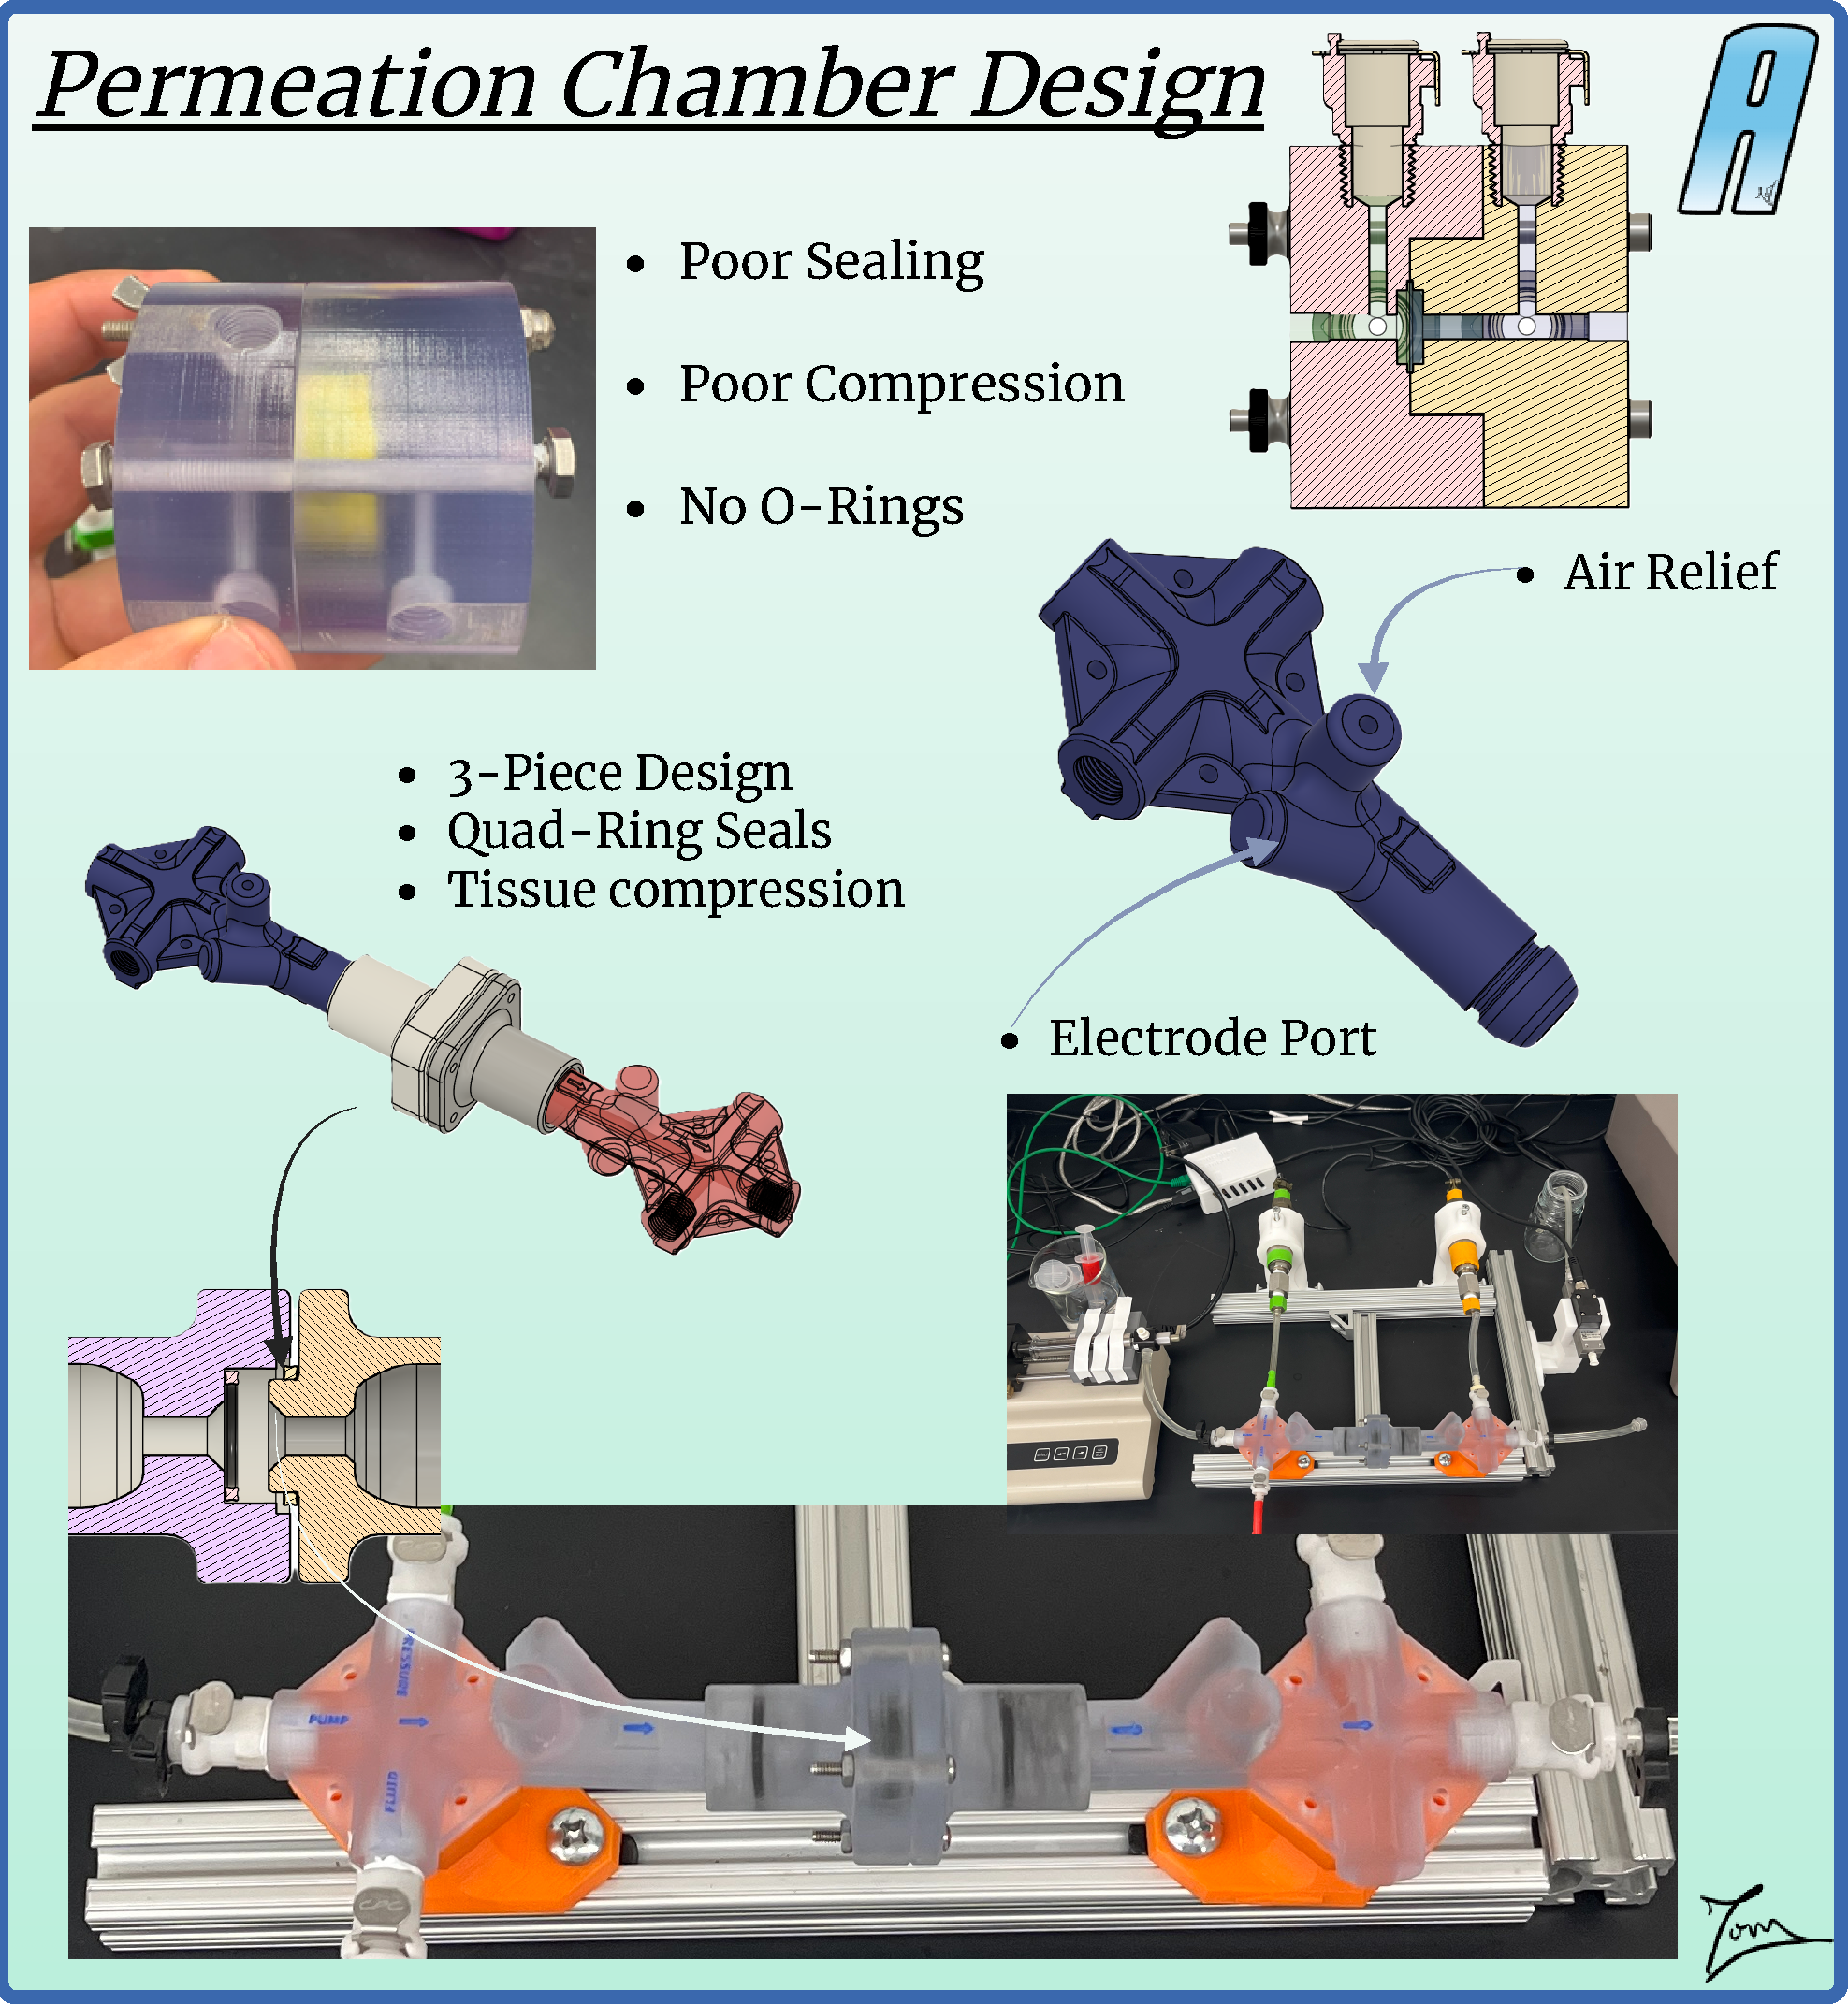
\includegraphics[width=1\linewidth]{figures/chapter 3/ch3_permCH.pdf}
    \caption[Iterative development of the permeation chamber design]{\textbf{Iterative development of the permeation chamber design.} The image outlines the evolution from an initial chamber with poor sealing and compression (top left) to an optimized 3-piece system featuring quad-ring seals, improved tissue compression, an air relief valve, and an electrode port for integrated monitoring. CAD renderings and assembly photos highlight key functional improvements, including enhanced sealing performance and modular construction to address early design limitations. }
    \label{fig:ch3_permCH}
\end{figure}
    
\subsection{Current Status and Future Directions}

While preliminary testing demonstrated successful fluid containment and basic functionality, full system validation awaits resolution of software integration challenges. The chamber design represents a significant advancement over traditional permeation testing systems, providing a robust foundation for comprehensive hydrogel permeability characterization~\cite{morejon2020compressiveproperties}. The enhanced measurement capabilities enable correlation with confined compression data, facilitating a more complete understanding of the relationship between mechanical properties and fluid transport characteristics in hydrated biomaterials~\cite{chaudhuri2016hydrogelstunable}.

The system's modular design and enhanced sealing capabilities make it particularly well-suited for assessing the effects of PCL scaffold architecture on permeability behavior~\cite{zhang20173dprintedpolyecaprolactone}. The integration of electrospun PCL membranes for porosity control can be systematically evaluated using this platform, providing insights into how synthetic reinforcement networks influence fluid transport properties in composite hydrogel systems~\cite{gao2018electrospunfiber}.

Future iterations will incorporate additional features including enhanced venting systems and potential integration of electrical property monitoring capabilities during permeation testing~\cite{woodruff2010returnforgotten}. The ability to simultaneously monitor electrical properties and permeability could provide valuable insights into the relationship between charge distribution and fluid transport in charged hydrogel systems~\cite{ahmed2015hydrogelpreparation}. This system thus lays essential groundwork for the accurate evaluation of next-generation tissue-engineered constructs under physiologically relevant conditions, where precise permeability measurements are crucial for predicting in vivo performance and ensuring successful tissue integration~\cite{kleinhans2018hydraulicpermeability}.

\section{Augmented via Additive: \protect\\ Establishing the Foundation}

This chapter established the foundational requirements for biomimetic meniscal tissue engineering through careful consideration of compositional, structural, and integration parameters. The development of an improved mechanical testing platform enabled precise characterization of these design requirements, providing quantitative targets for scaffold development. By defining specific criteria for water content, matrix distribution, and hierarchical organization, and mechanical properties we have created a robust framework for evaluating PCL-reinforced hydrogel constructs.

The next chapter, "Additive Network Integration (A + N + I)," builds upon these established requirements by exploring how advanced manufacturing techniques can be leveraged to create precisely controlled PCL reinforcement networks. Through strategic implementation of additive manufacturing approaches, we investigate methods to achieve the compositional and structural targets outlined here while maintaining the critical integration requirements necessary for proper mechanical function. This systematic progression from design criteria to fabrication strategy represents a crucial step toward developing clinically relevant meniscal replacements.